Distribution for the GNN input variables in the inclusive signal region with a cut on the GNN score (GNN-score>0.7) are shown in \ref{GNN_input_modelling_1} and \ref{GNN_input_modelling_2}, which show the regions of the phase space where the signal mostly concentrates in. The reasonability of the modelling after GNN discrimination can be verified with checking the distributions of the signal-rich regions in \ref{app:validation_GNN_input_1L_ge10j4b}. For instance, signal is mostly located in region (0.5, 1.6) for the variable dRbb\_MindR\_DL1r\_70. Then the modelling is reasonable in that region from the distribution in 1L ge10j4b.

\begin{figure}

        \begin{center} \setlength{\tabcolsep}{2.5pt}\footnotesize
        \begin{tabular}{cccc}
        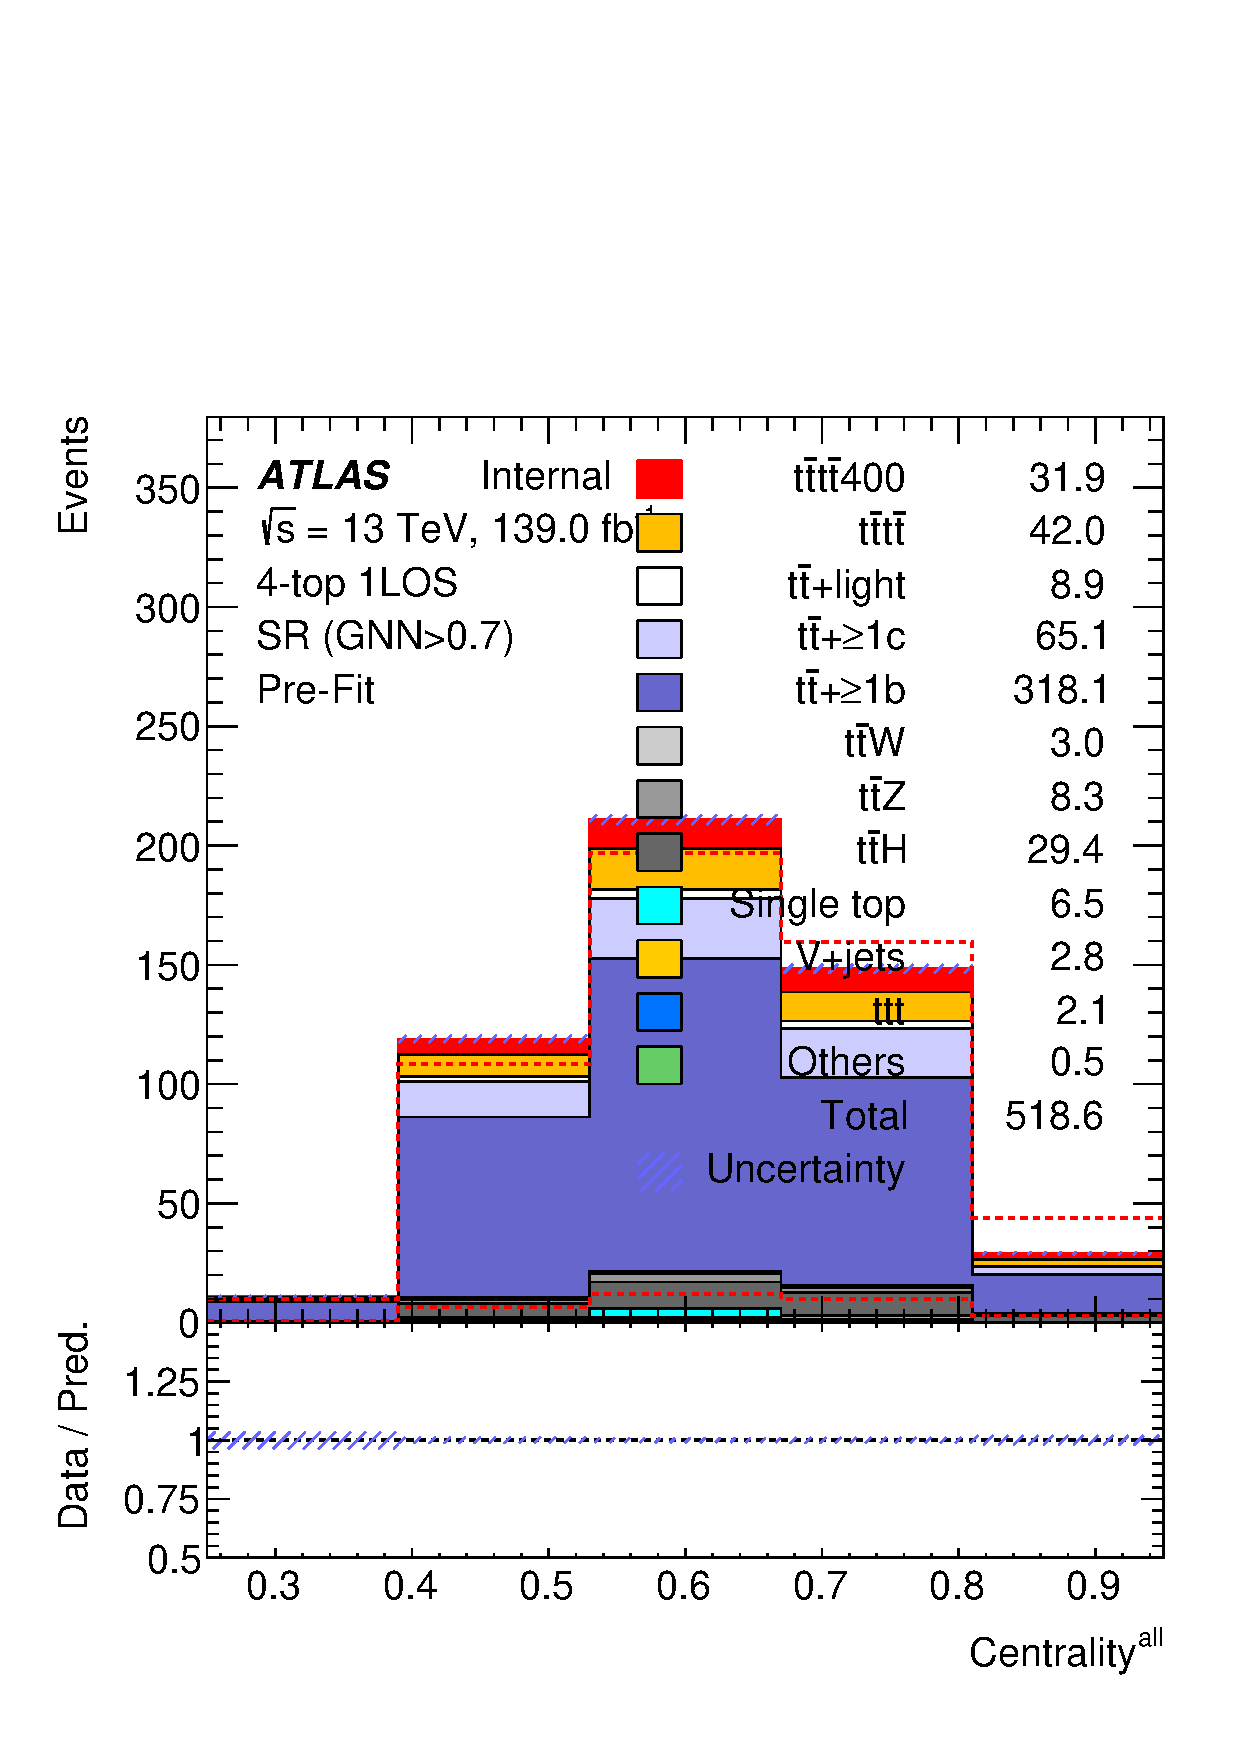
\includegraphics[width=0.23 \textwidth]{figures/gnn/Modeling/Centrality_all.pdf} &
        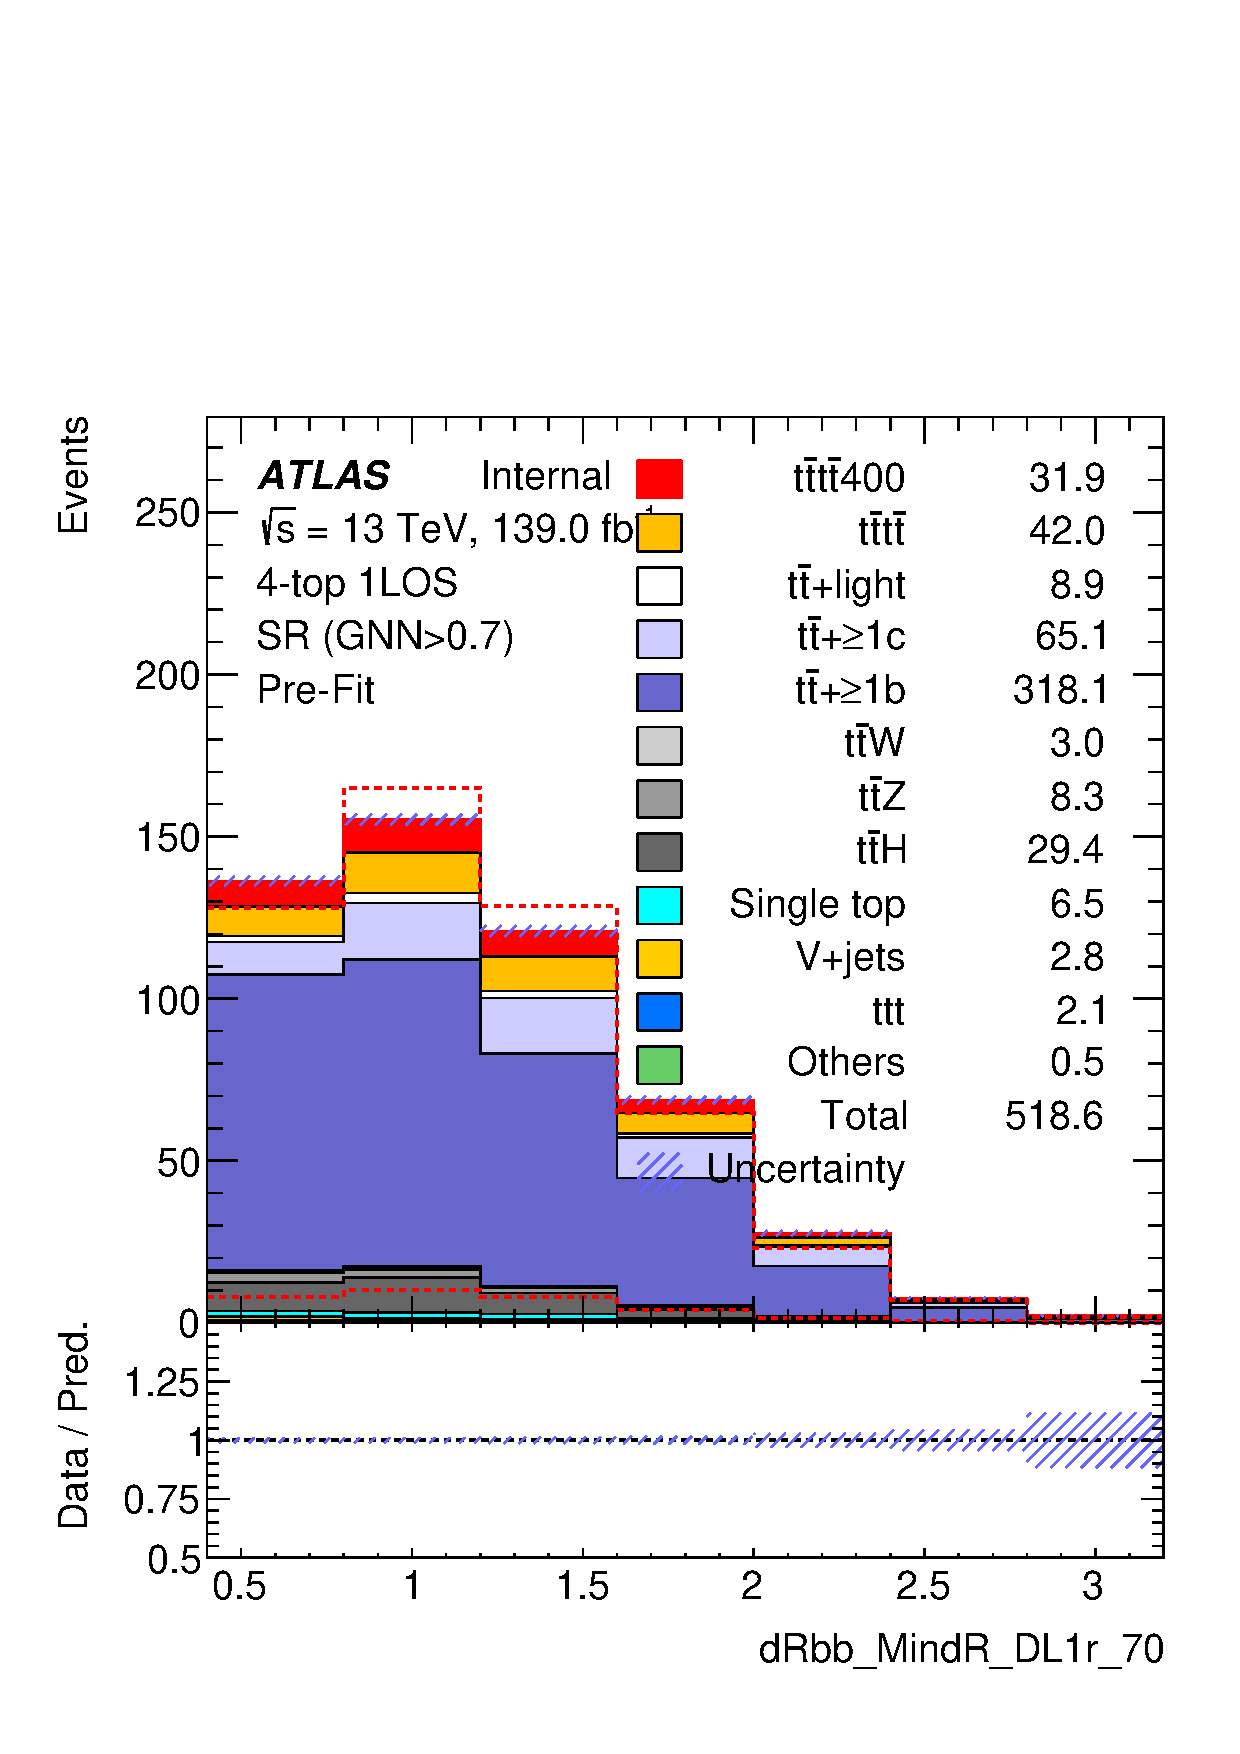
\includegraphics[width=0.23 \textwidth]{figures/gnn/Modeling/dRbb_MindR_DL1r_70.pdf} &
        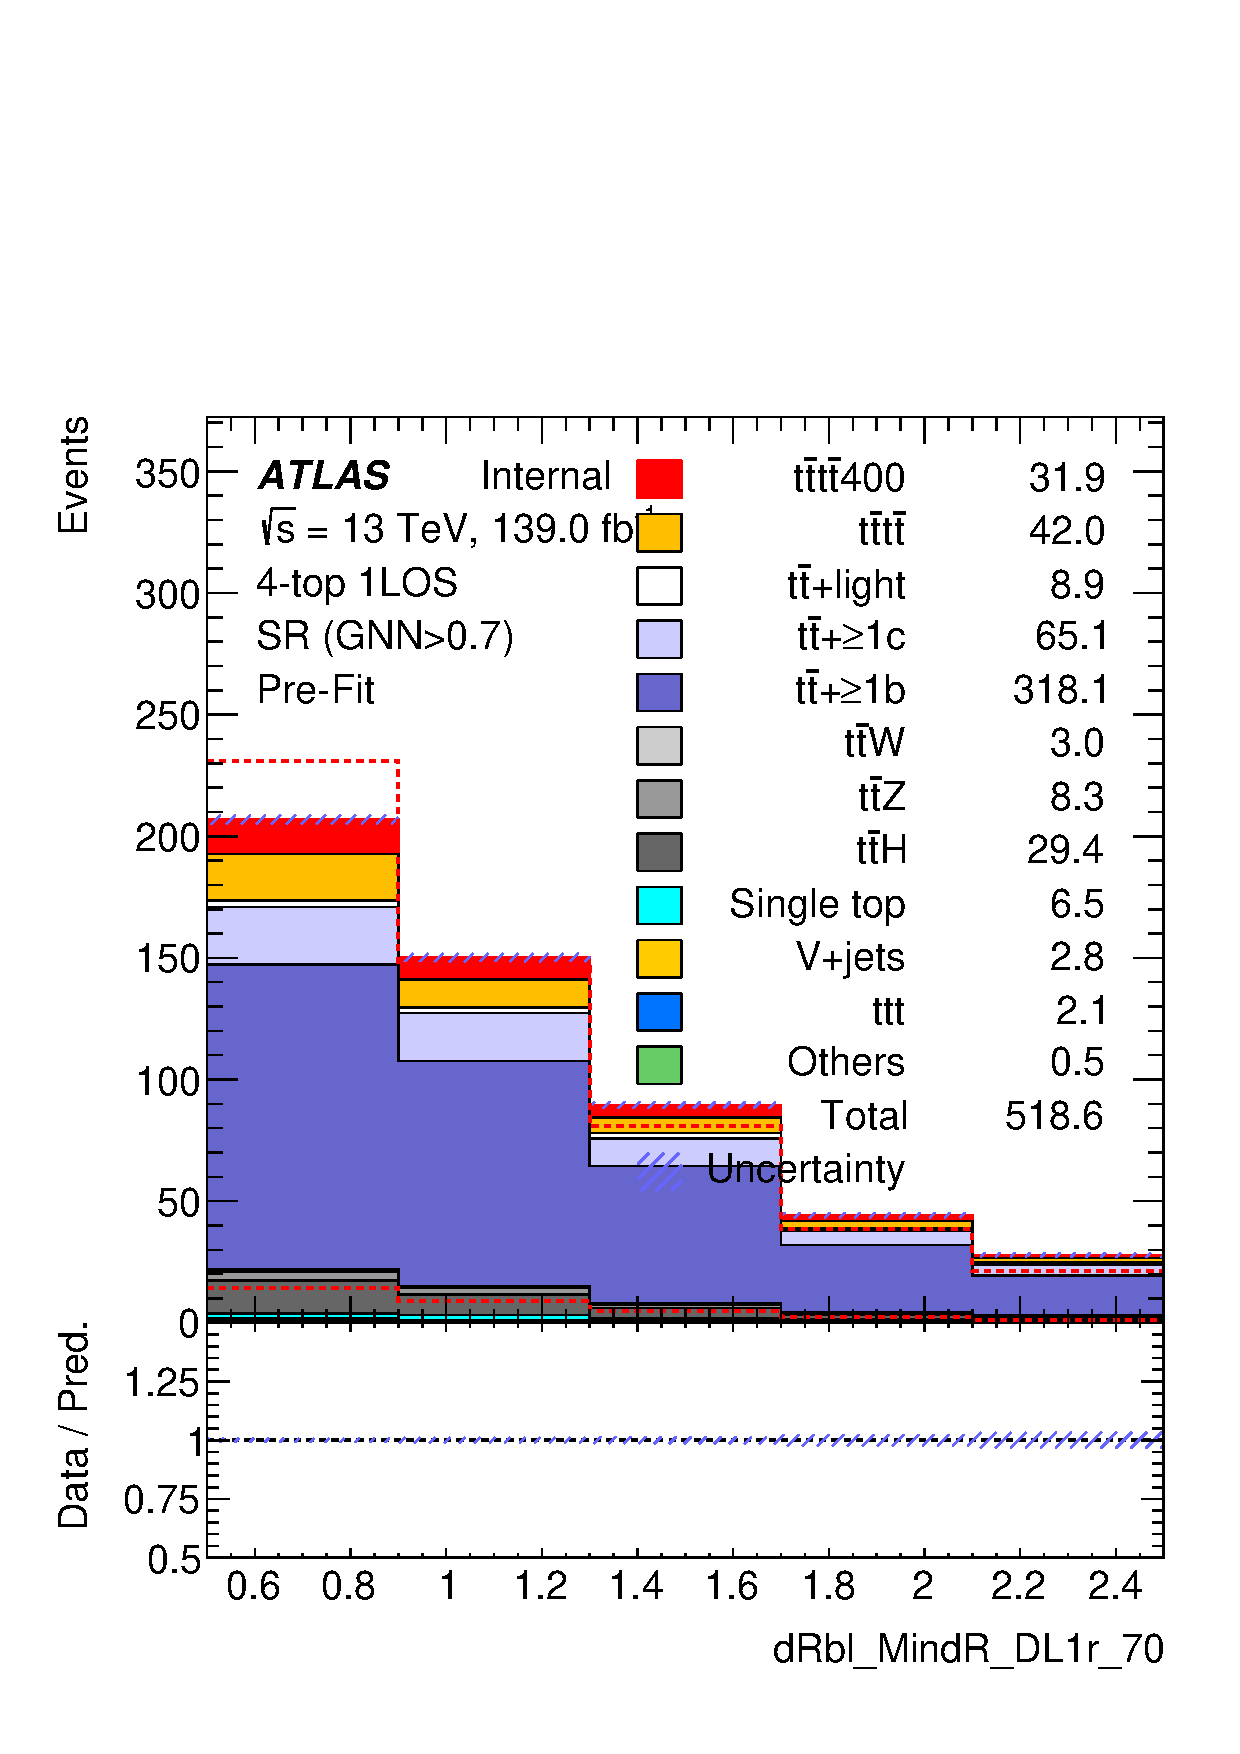
\includegraphics[width=0.23 \textwidth]{figures/gnn/Modeling/dRbl_MindR_DL1r_70.pdf} &
        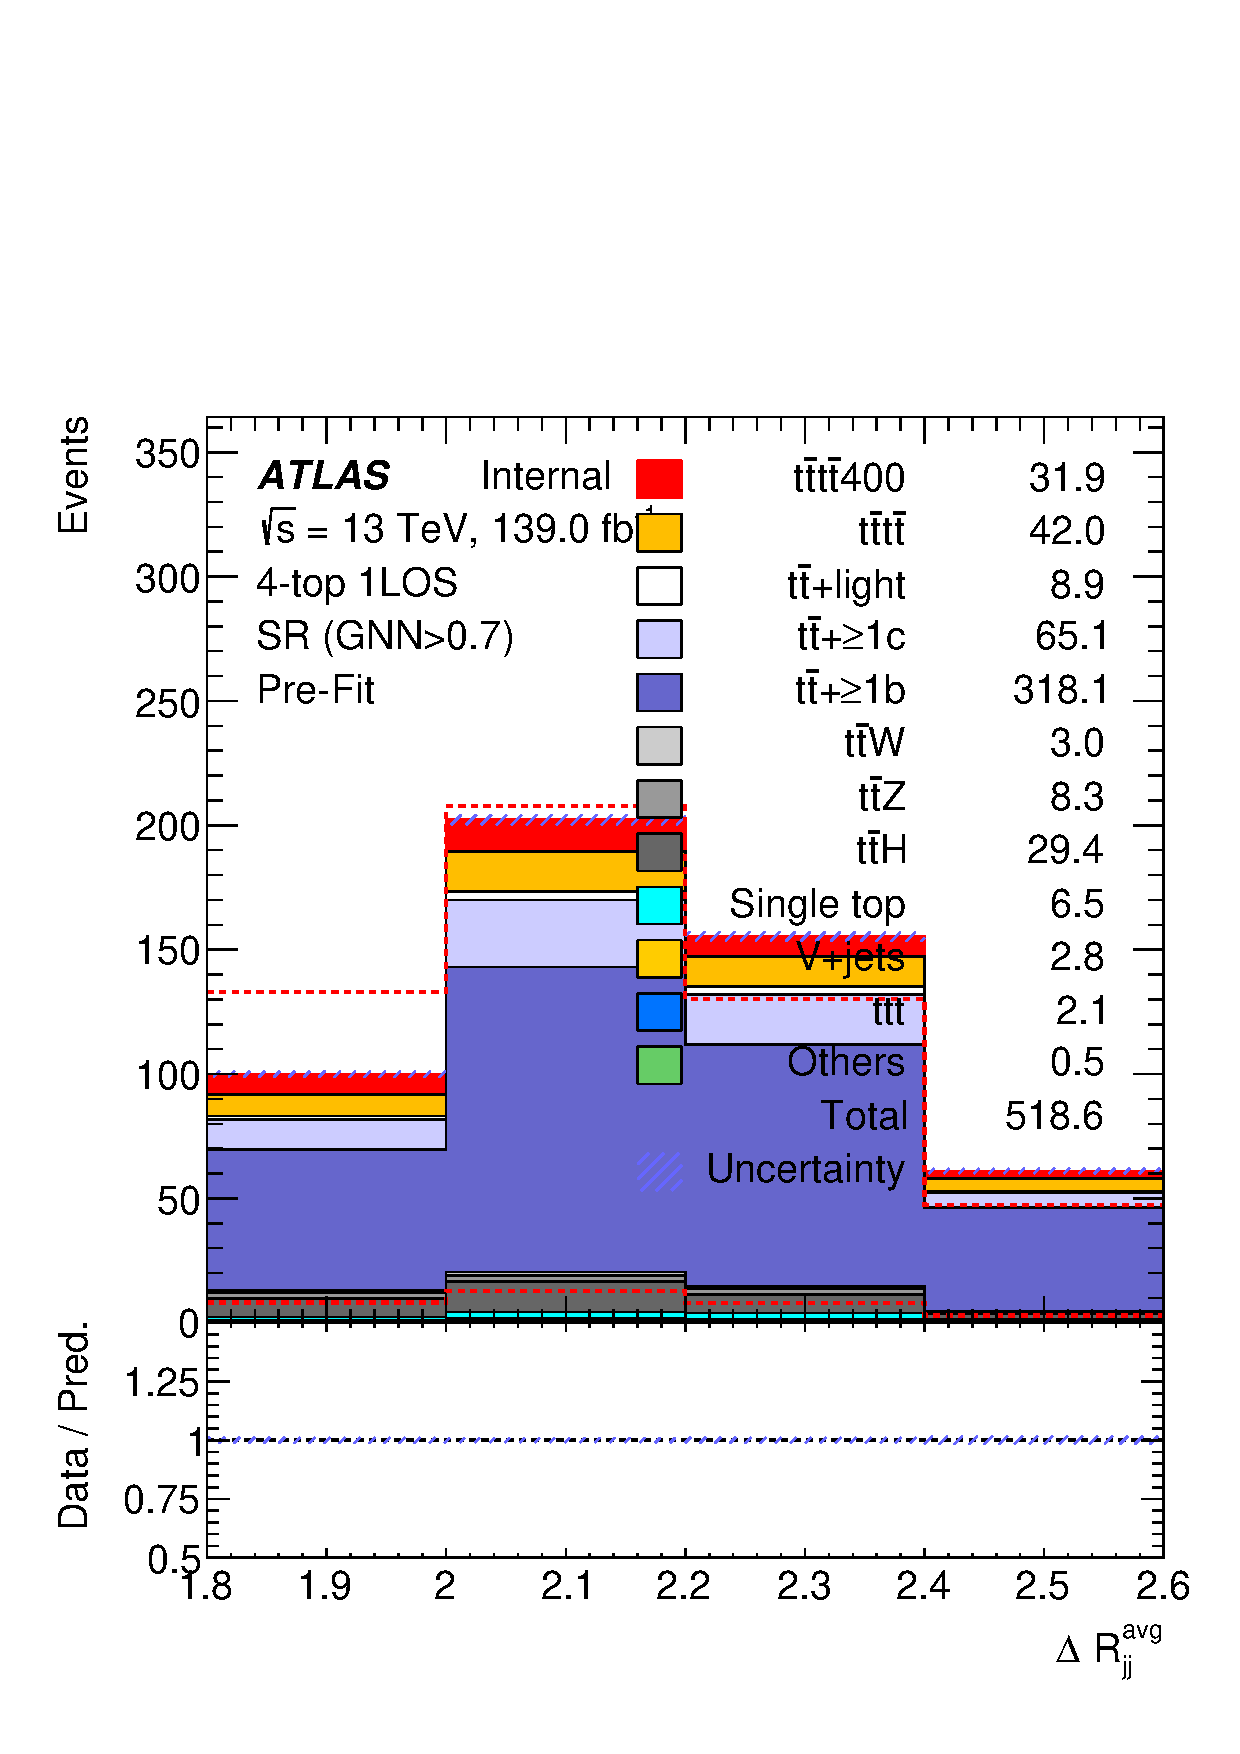
\includegraphics[width=0.23 \textwidth]{figures/gnn/Modeling/dRjj_Avg.pdf}\\


        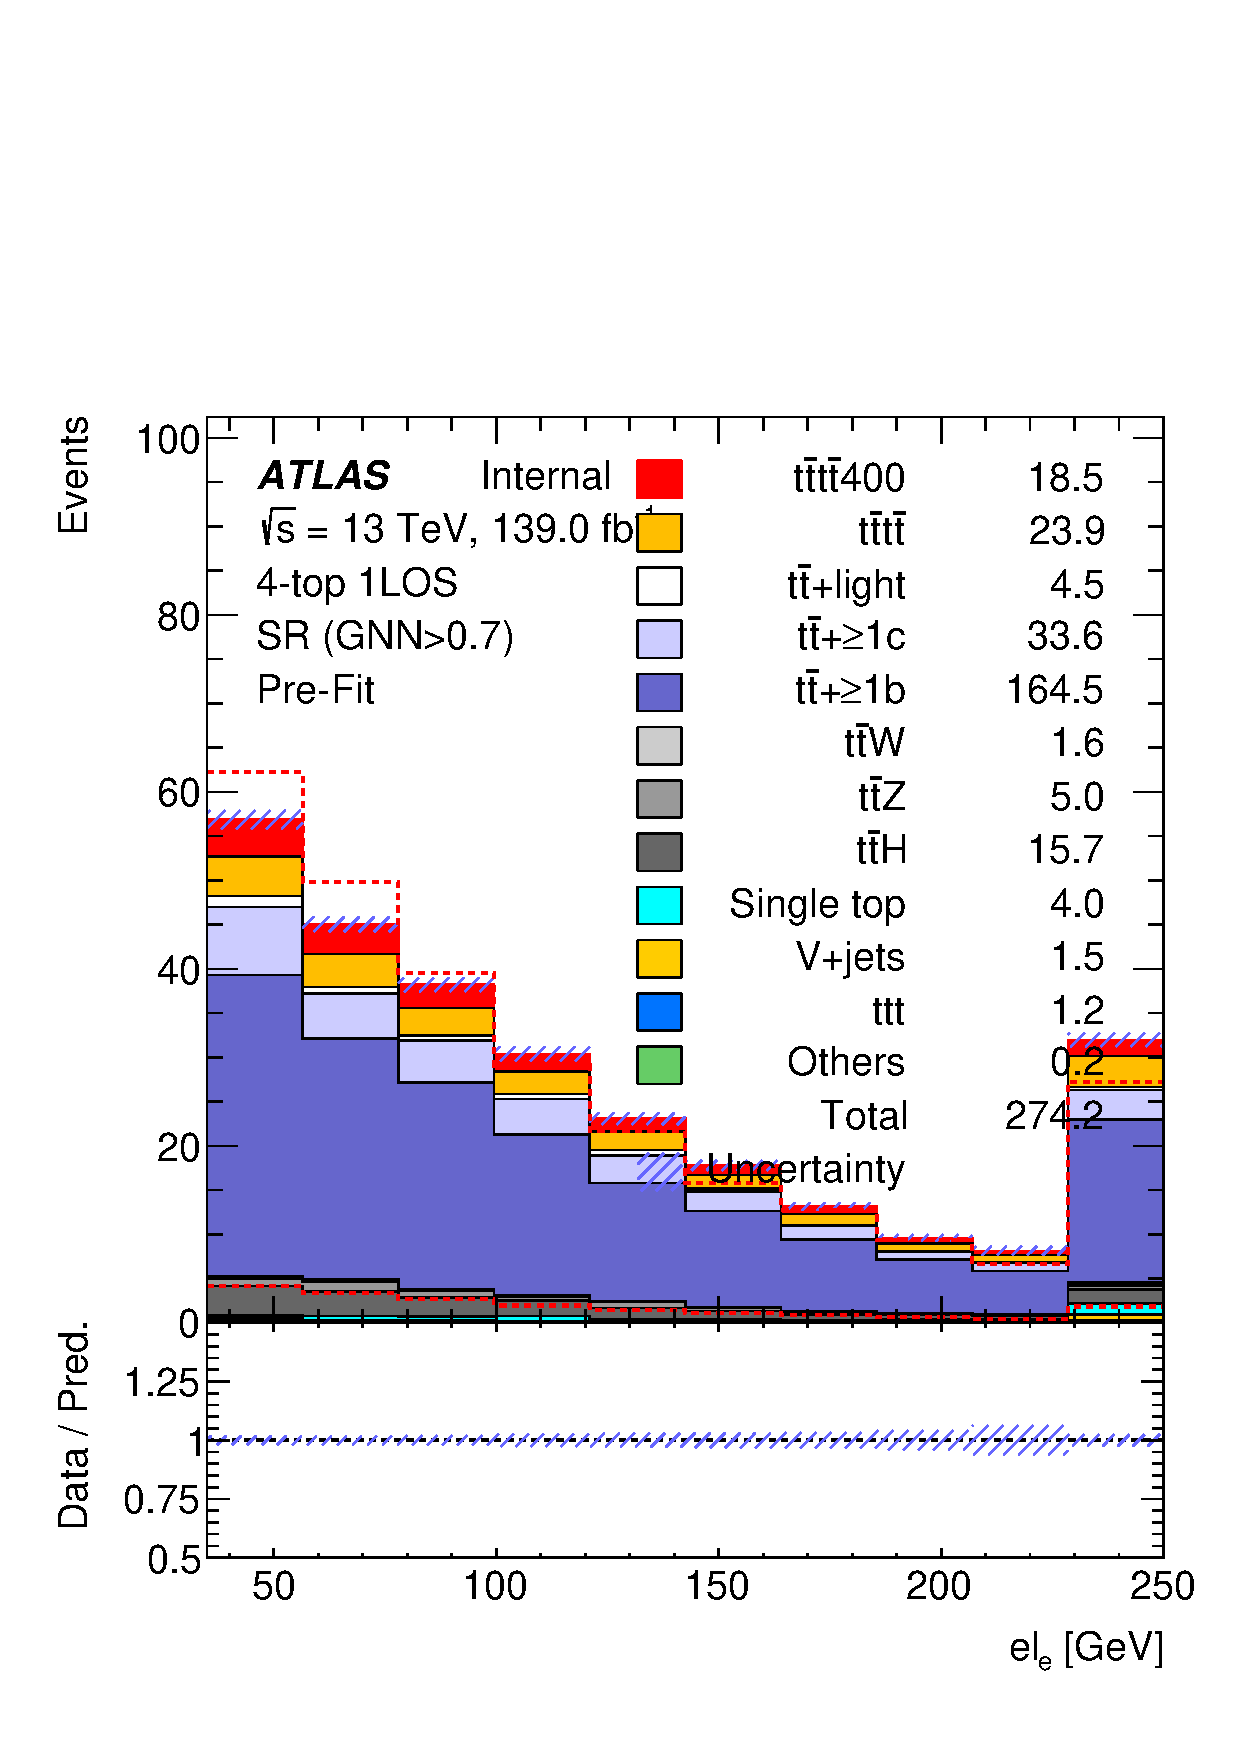
\includegraphics[width=0.23 \textwidth]{figures/gnn/Modeling/el_e.pdf} &
        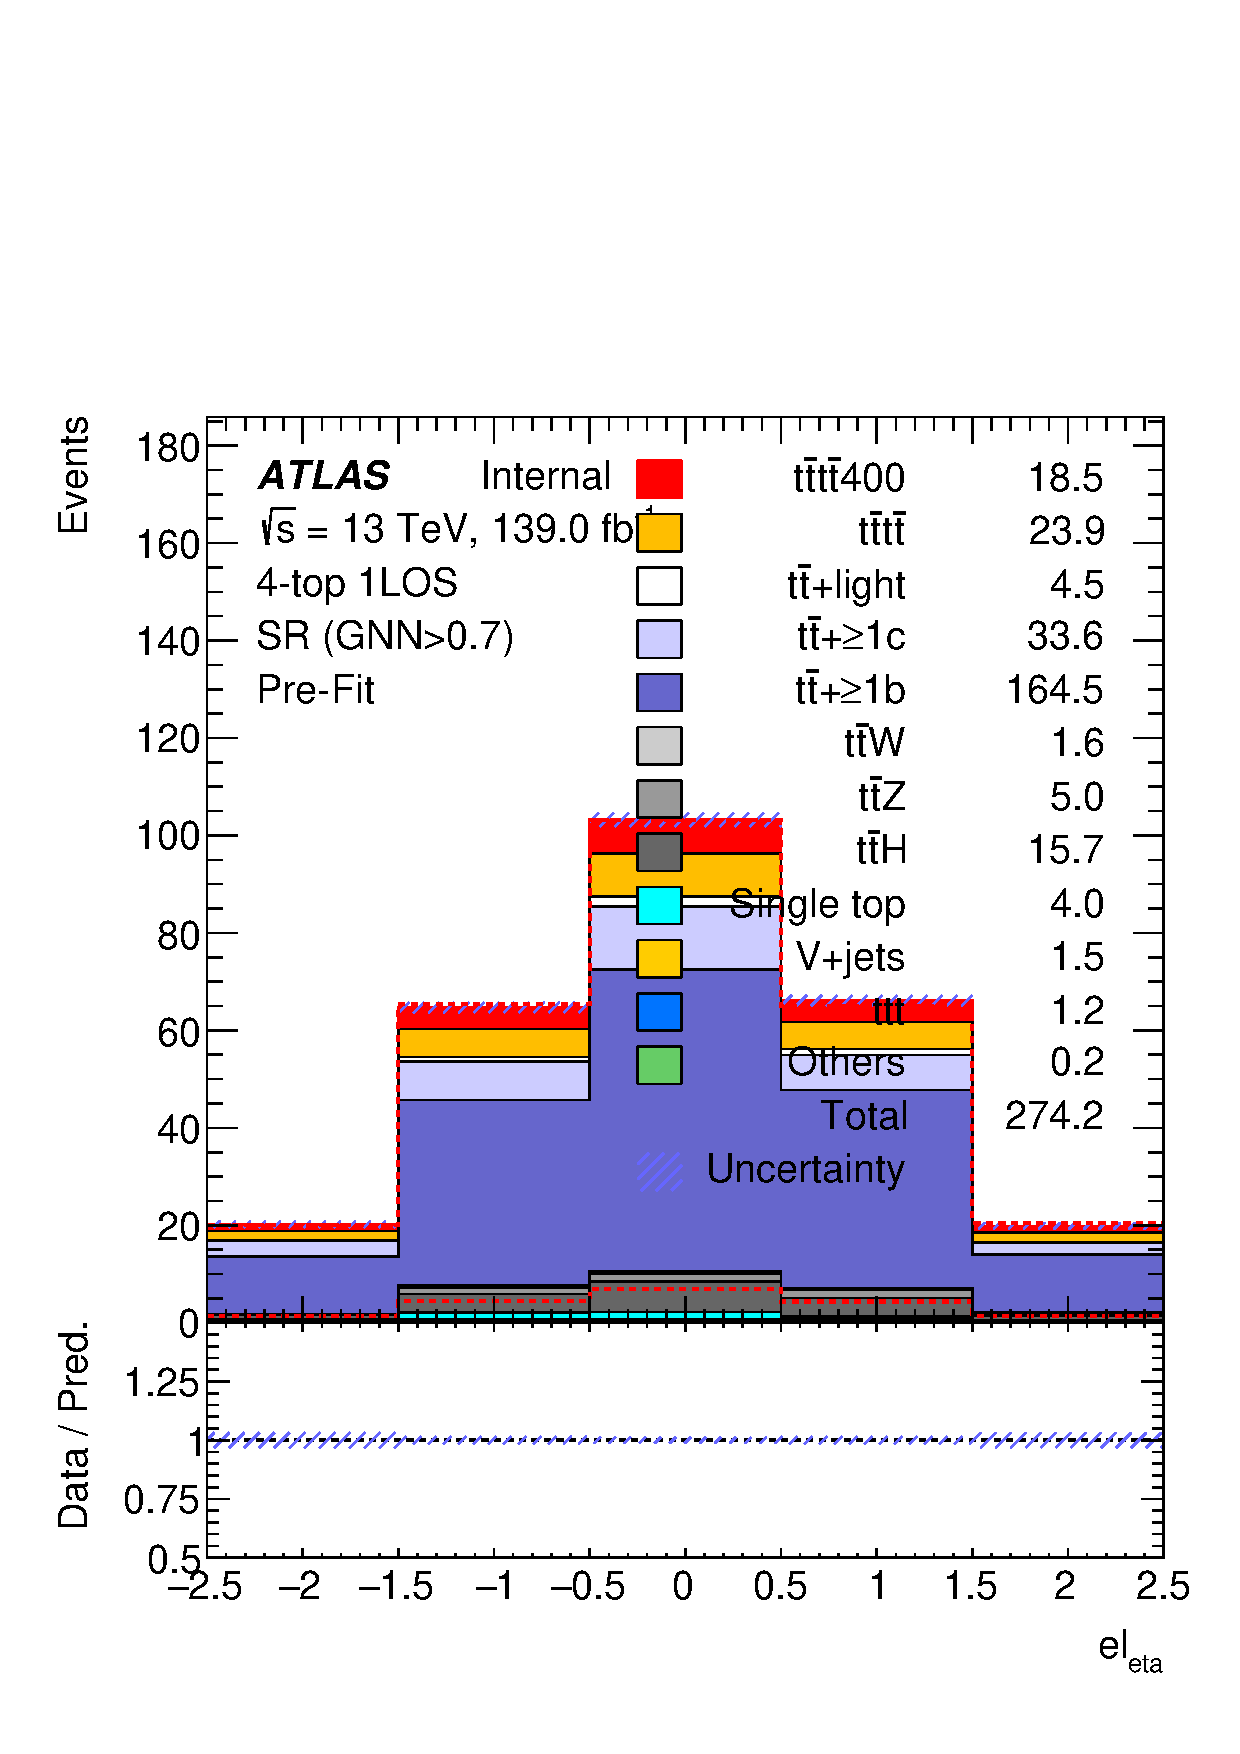
\includegraphics[width=0.23 \textwidth]{figures/gnn/Modeling/el_eta.pdf} &
        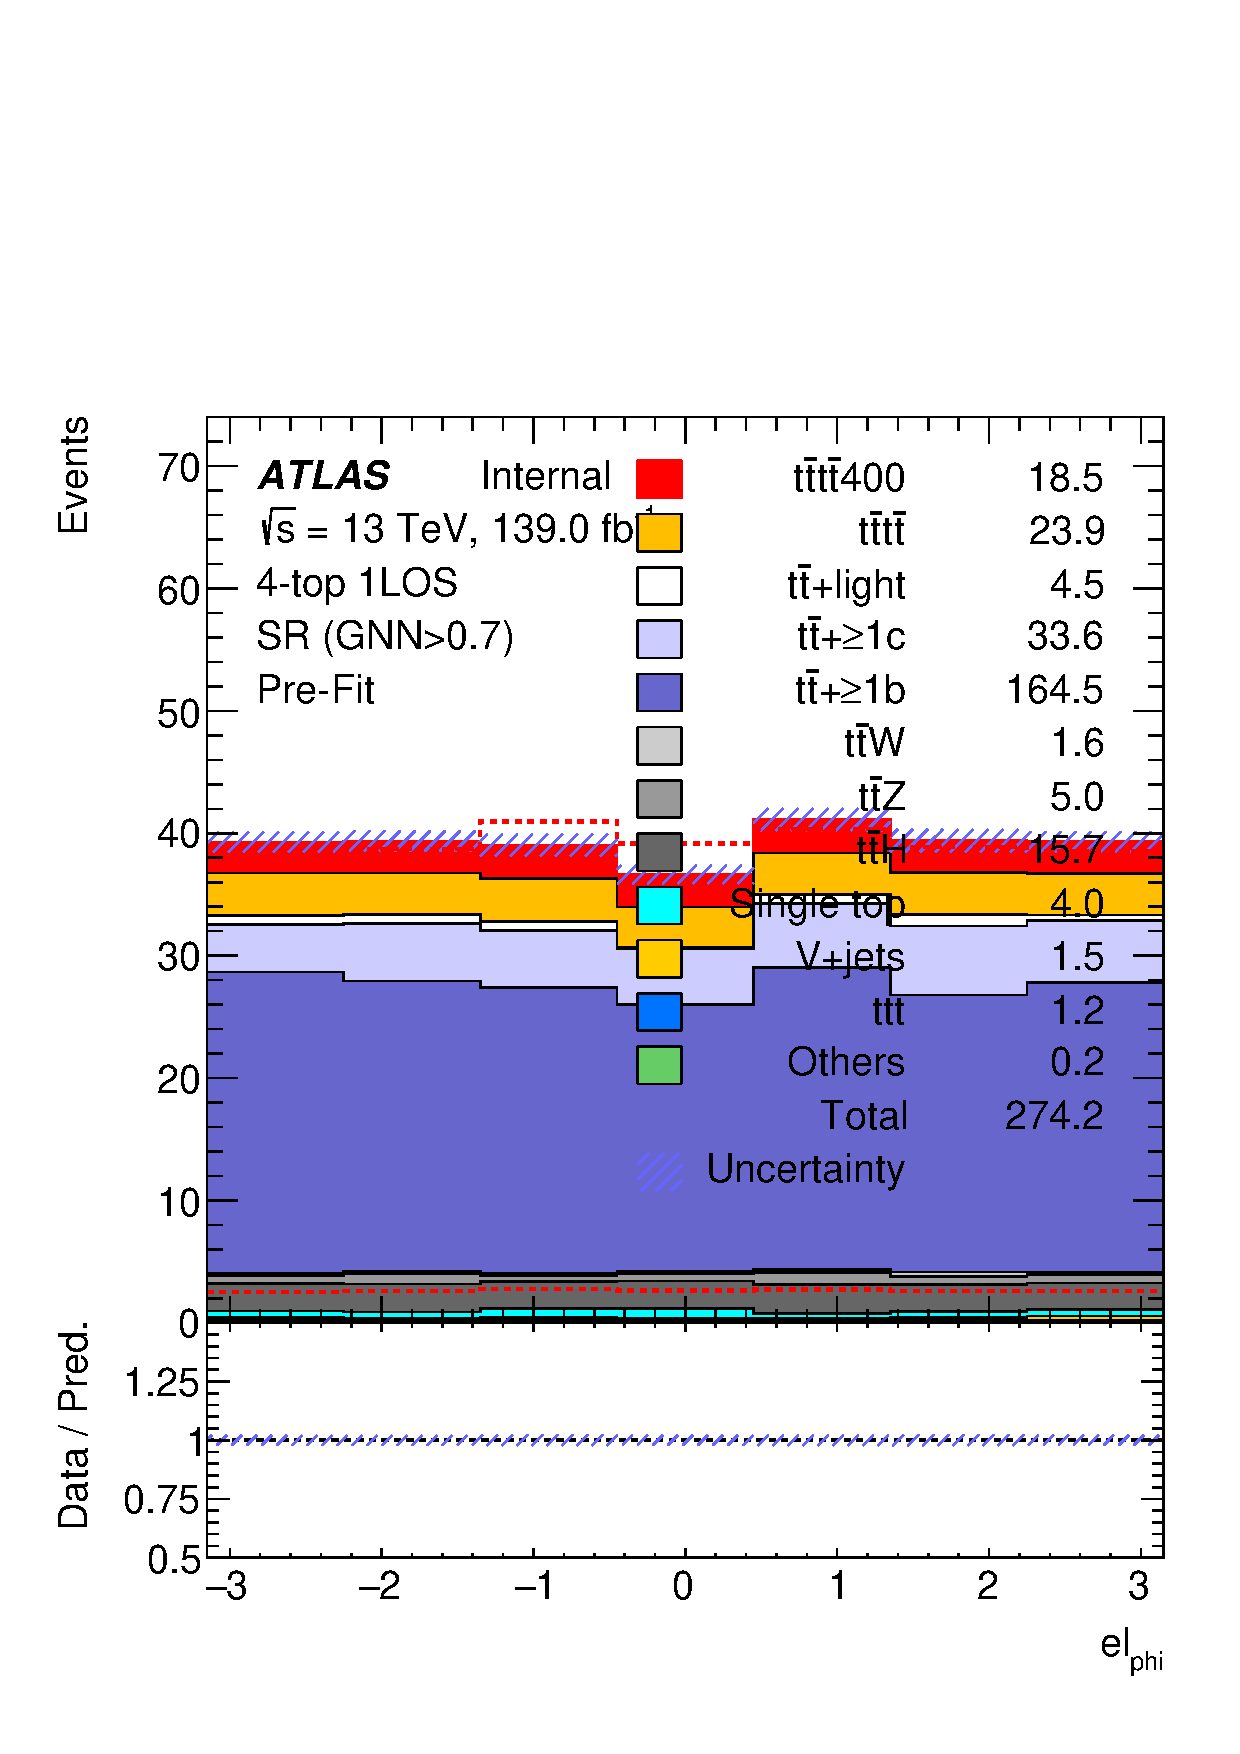
\includegraphics[width=0.23 \textwidth]{figures/gnn/Modeling/el_phi.pdf} &
        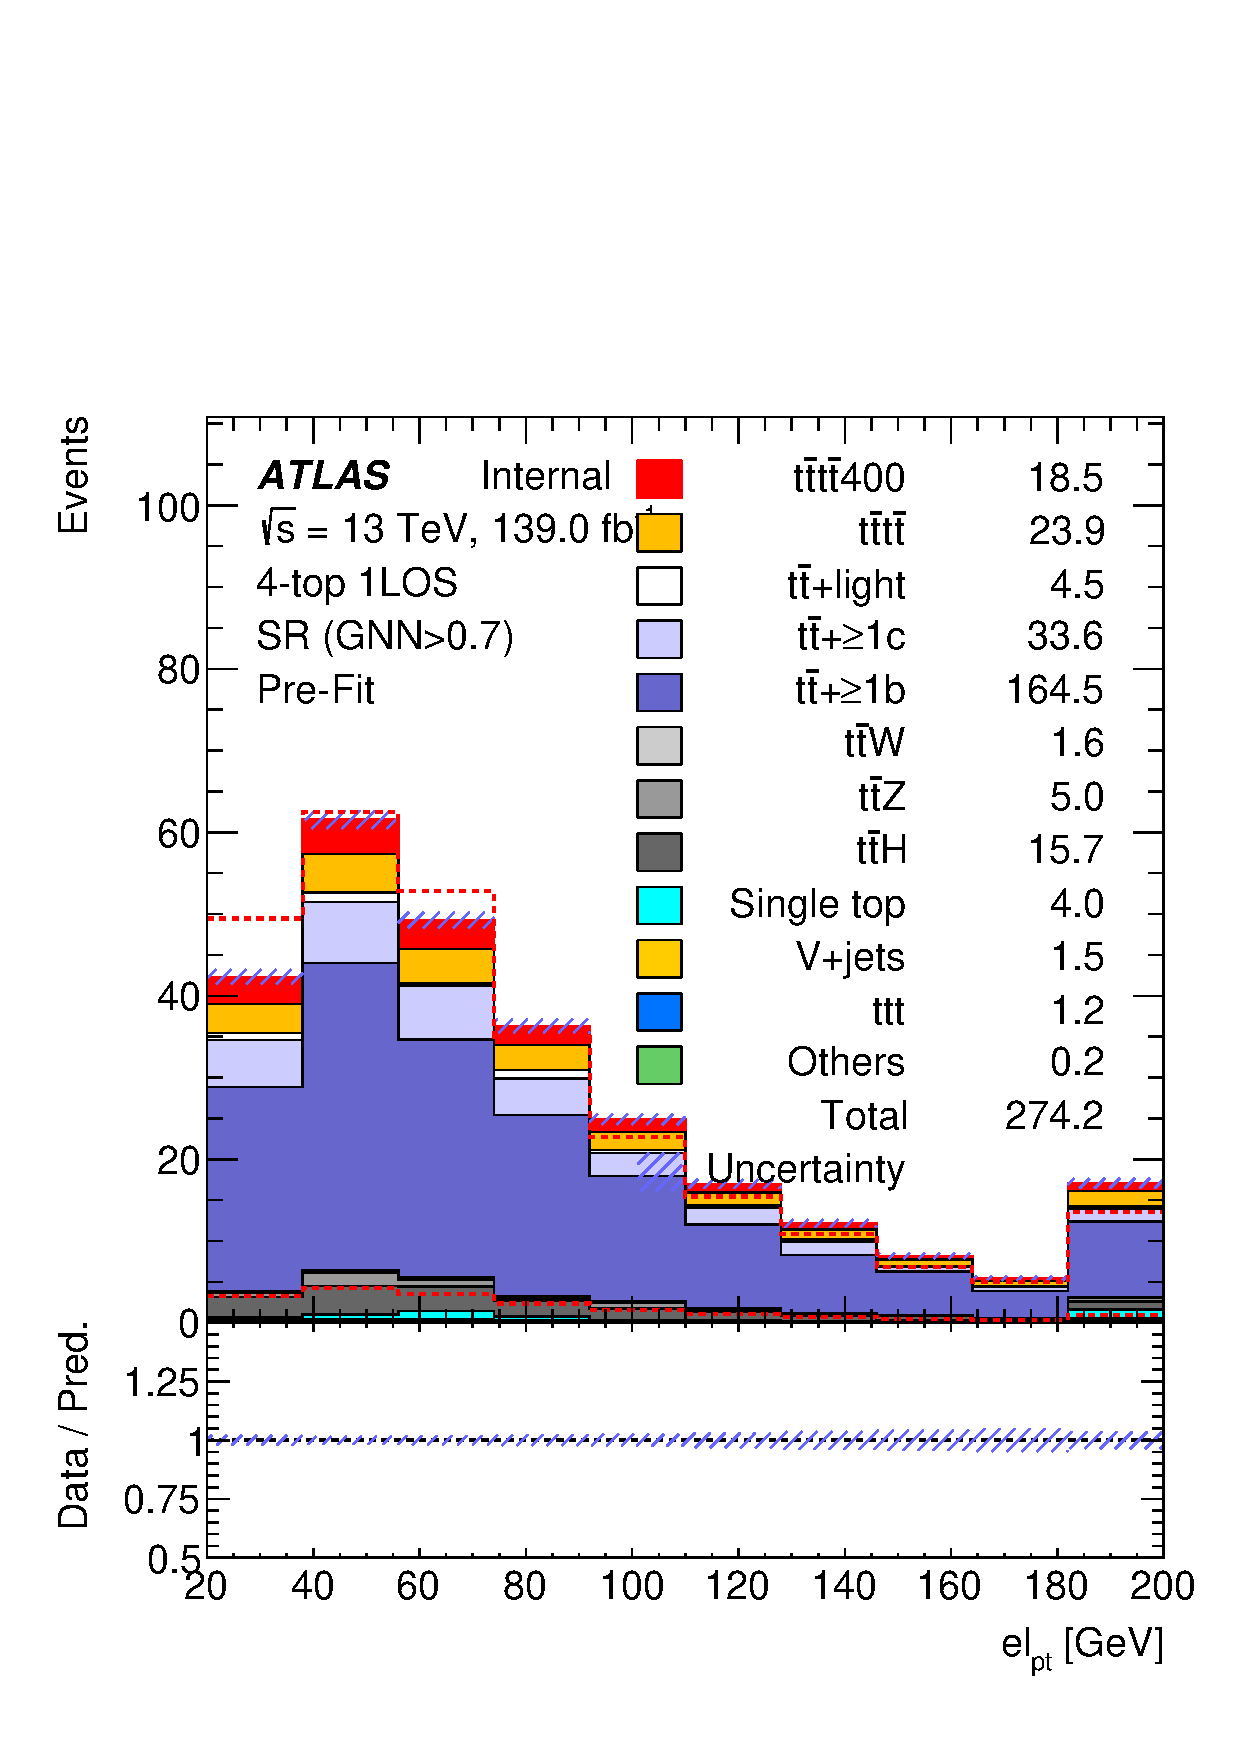
\includegraphics[width=0.23 \textwidth]{figures/gnn/Modeling/el_pt.pdf} \\

        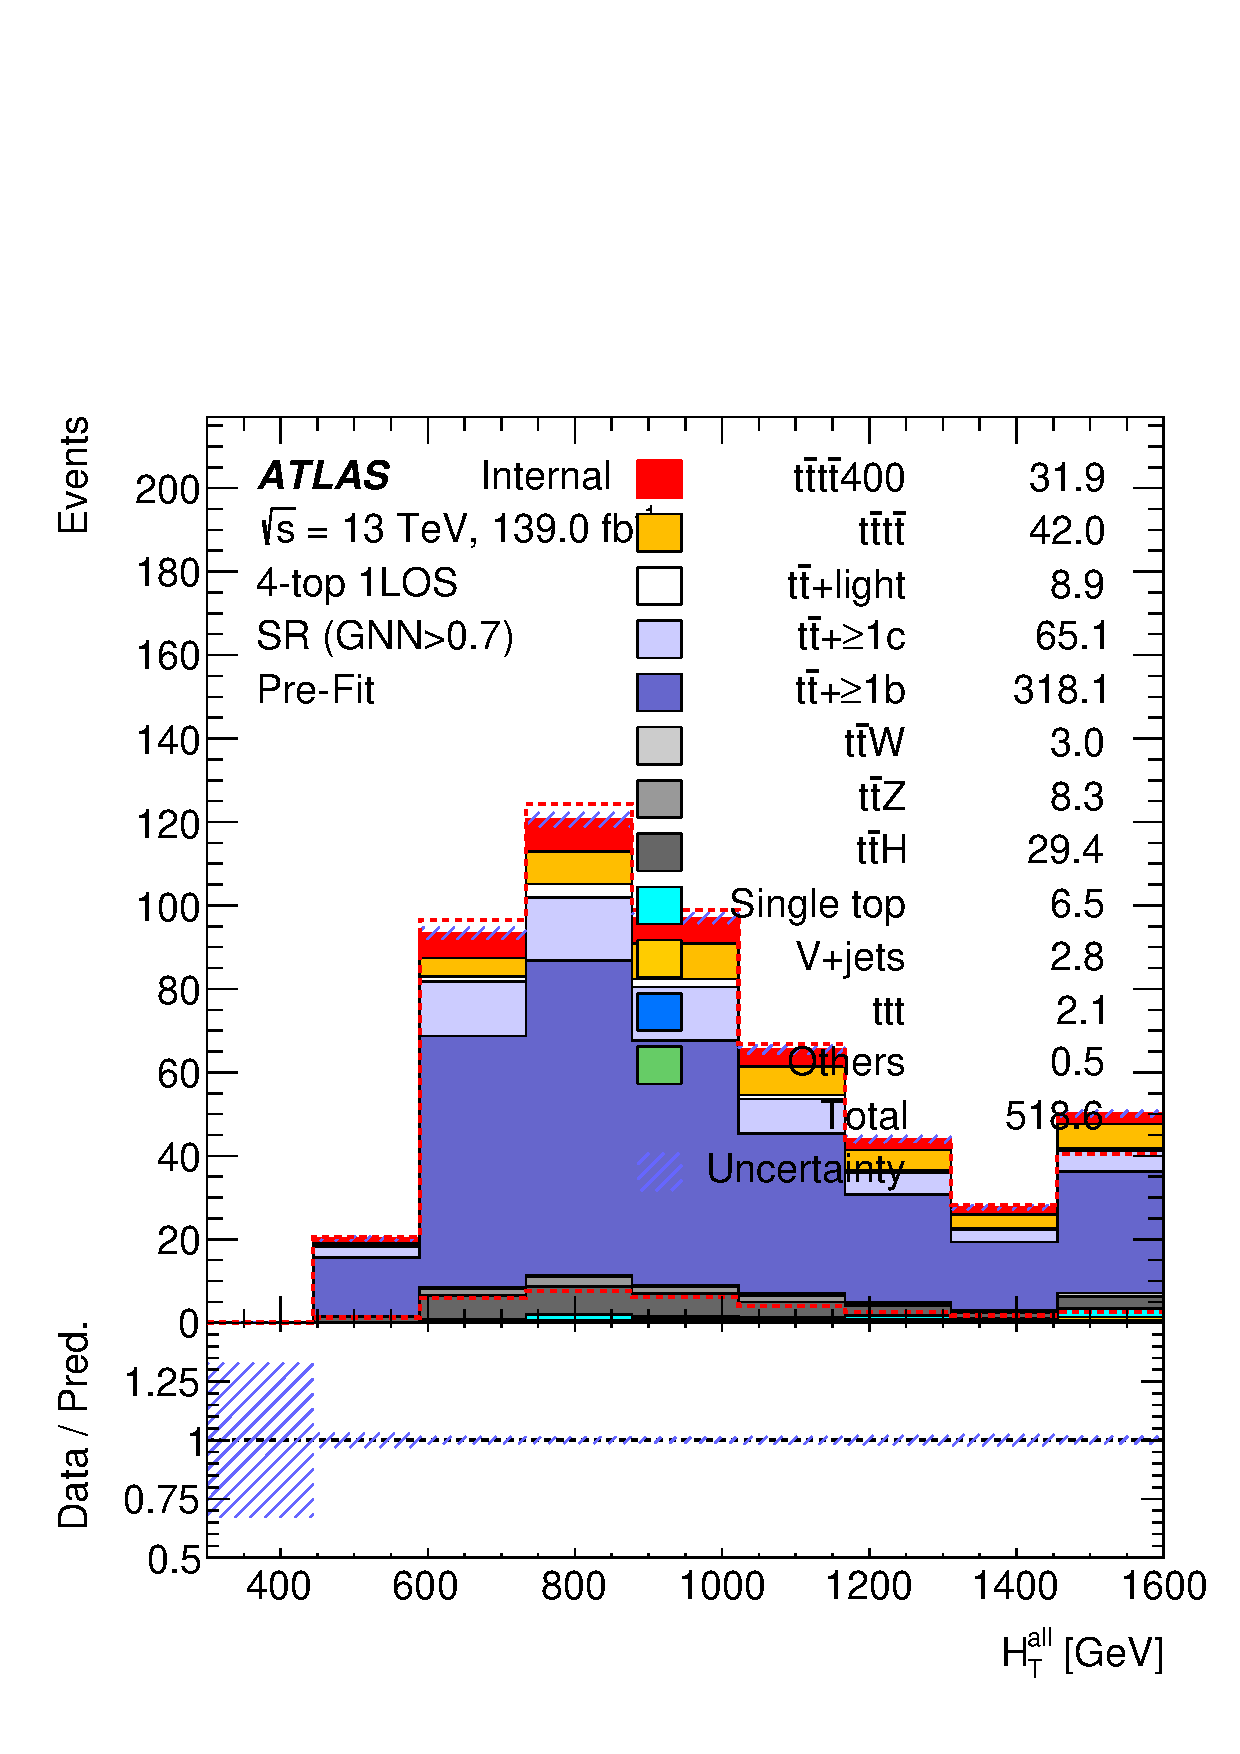
\includegraphics[width=0.23 \textwidth]{figures/gnn/Modeling/HT.pdf} &
        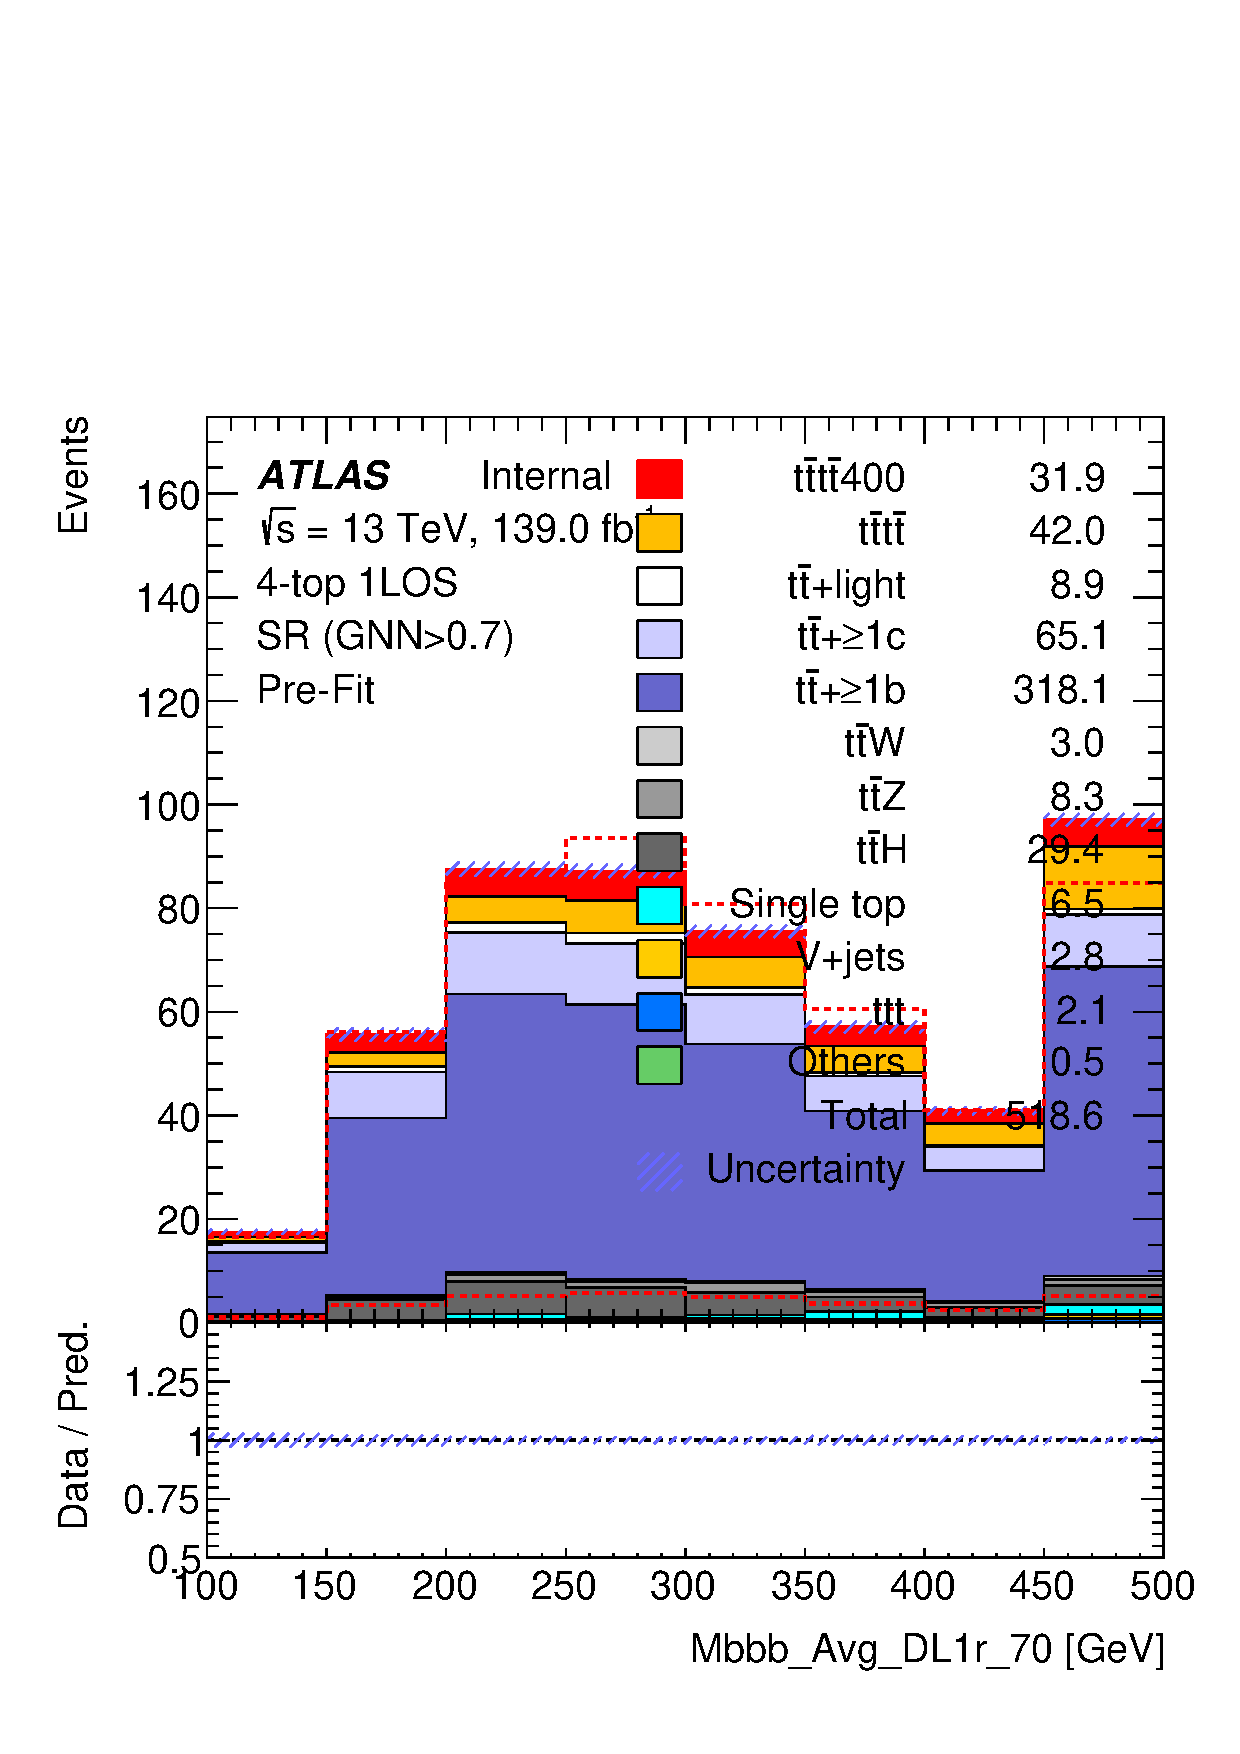
\includegraphics[width=0.23 \textwidth]{figures/gnn/Modeling/Mbbb_Avg_DL1r_70.pdf} &
        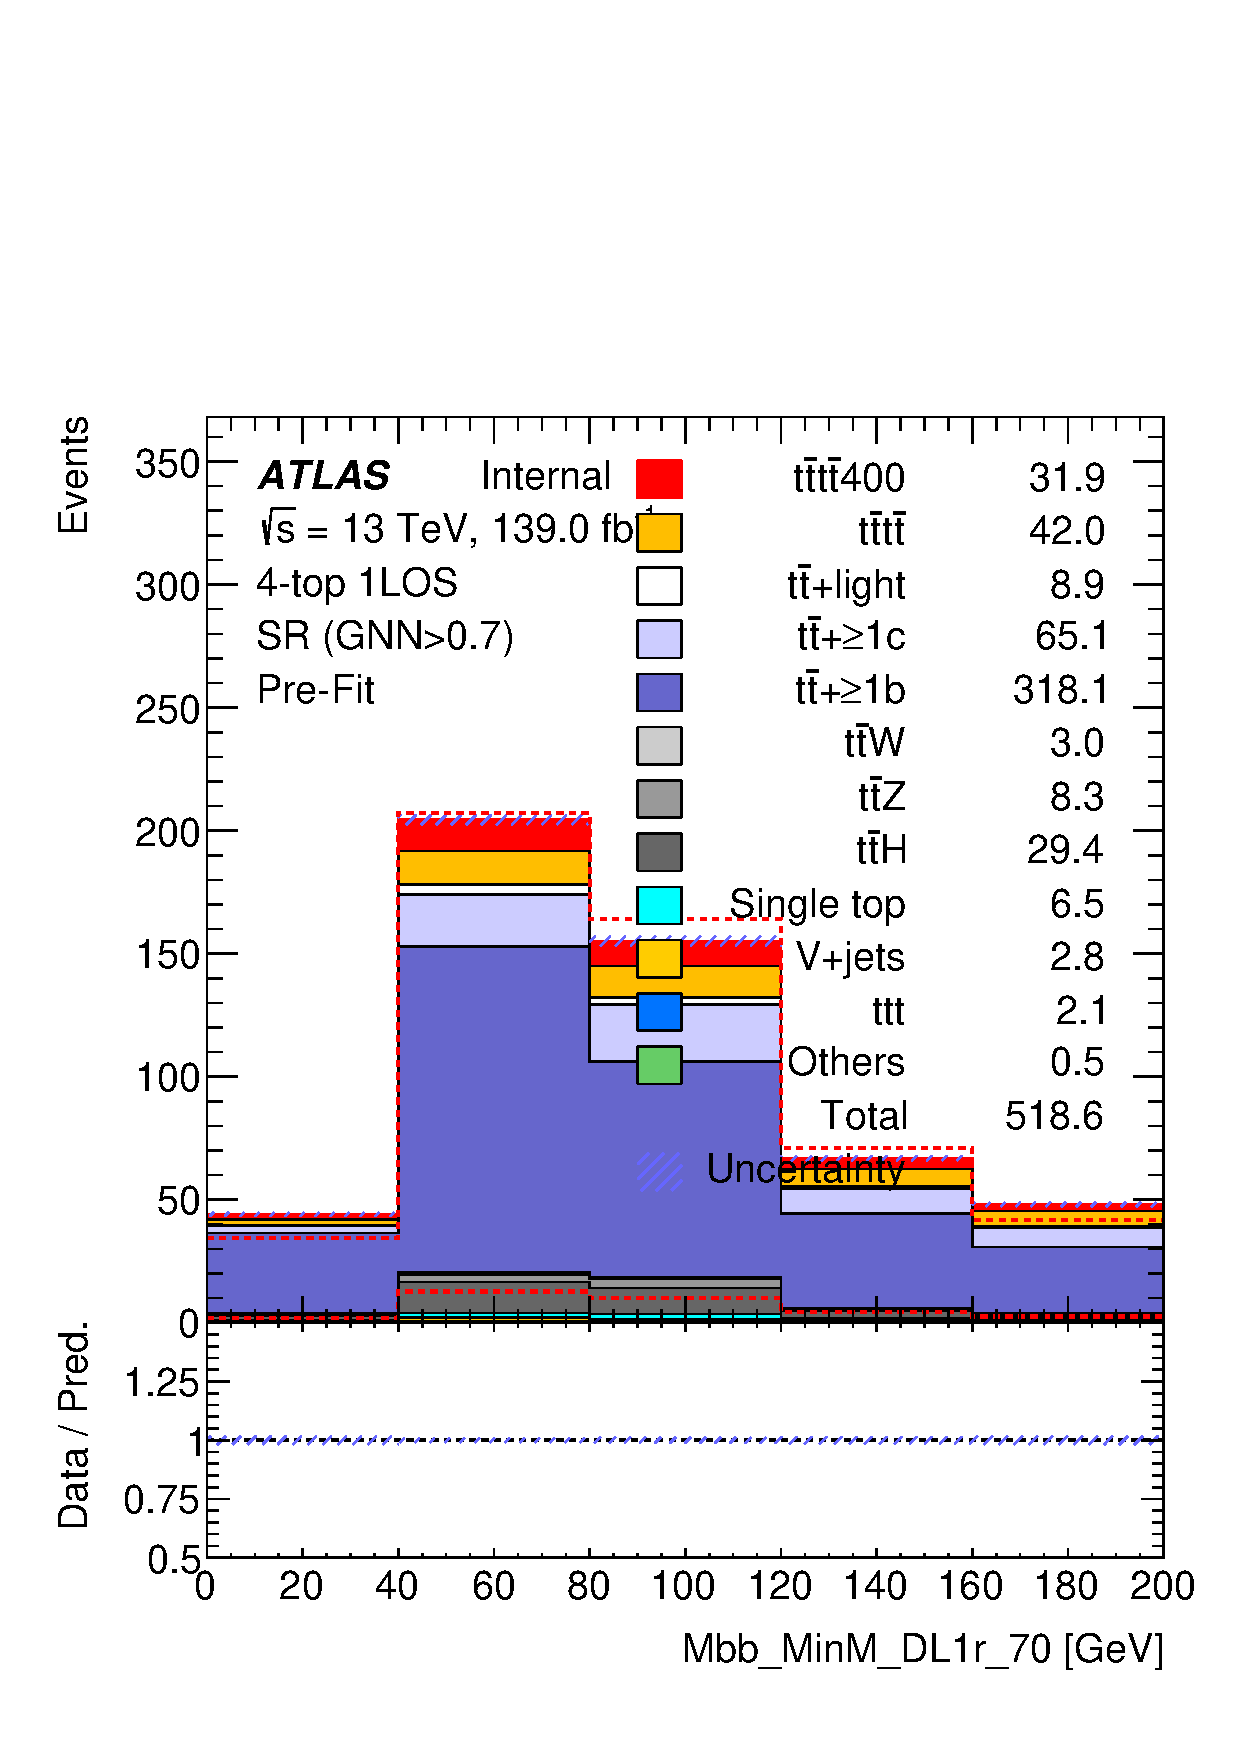
\includegraphics[width=0.23 \textwidth]{figures/gnn/Modeling/Mbb_MinM_DL1r_70.pdf} &
        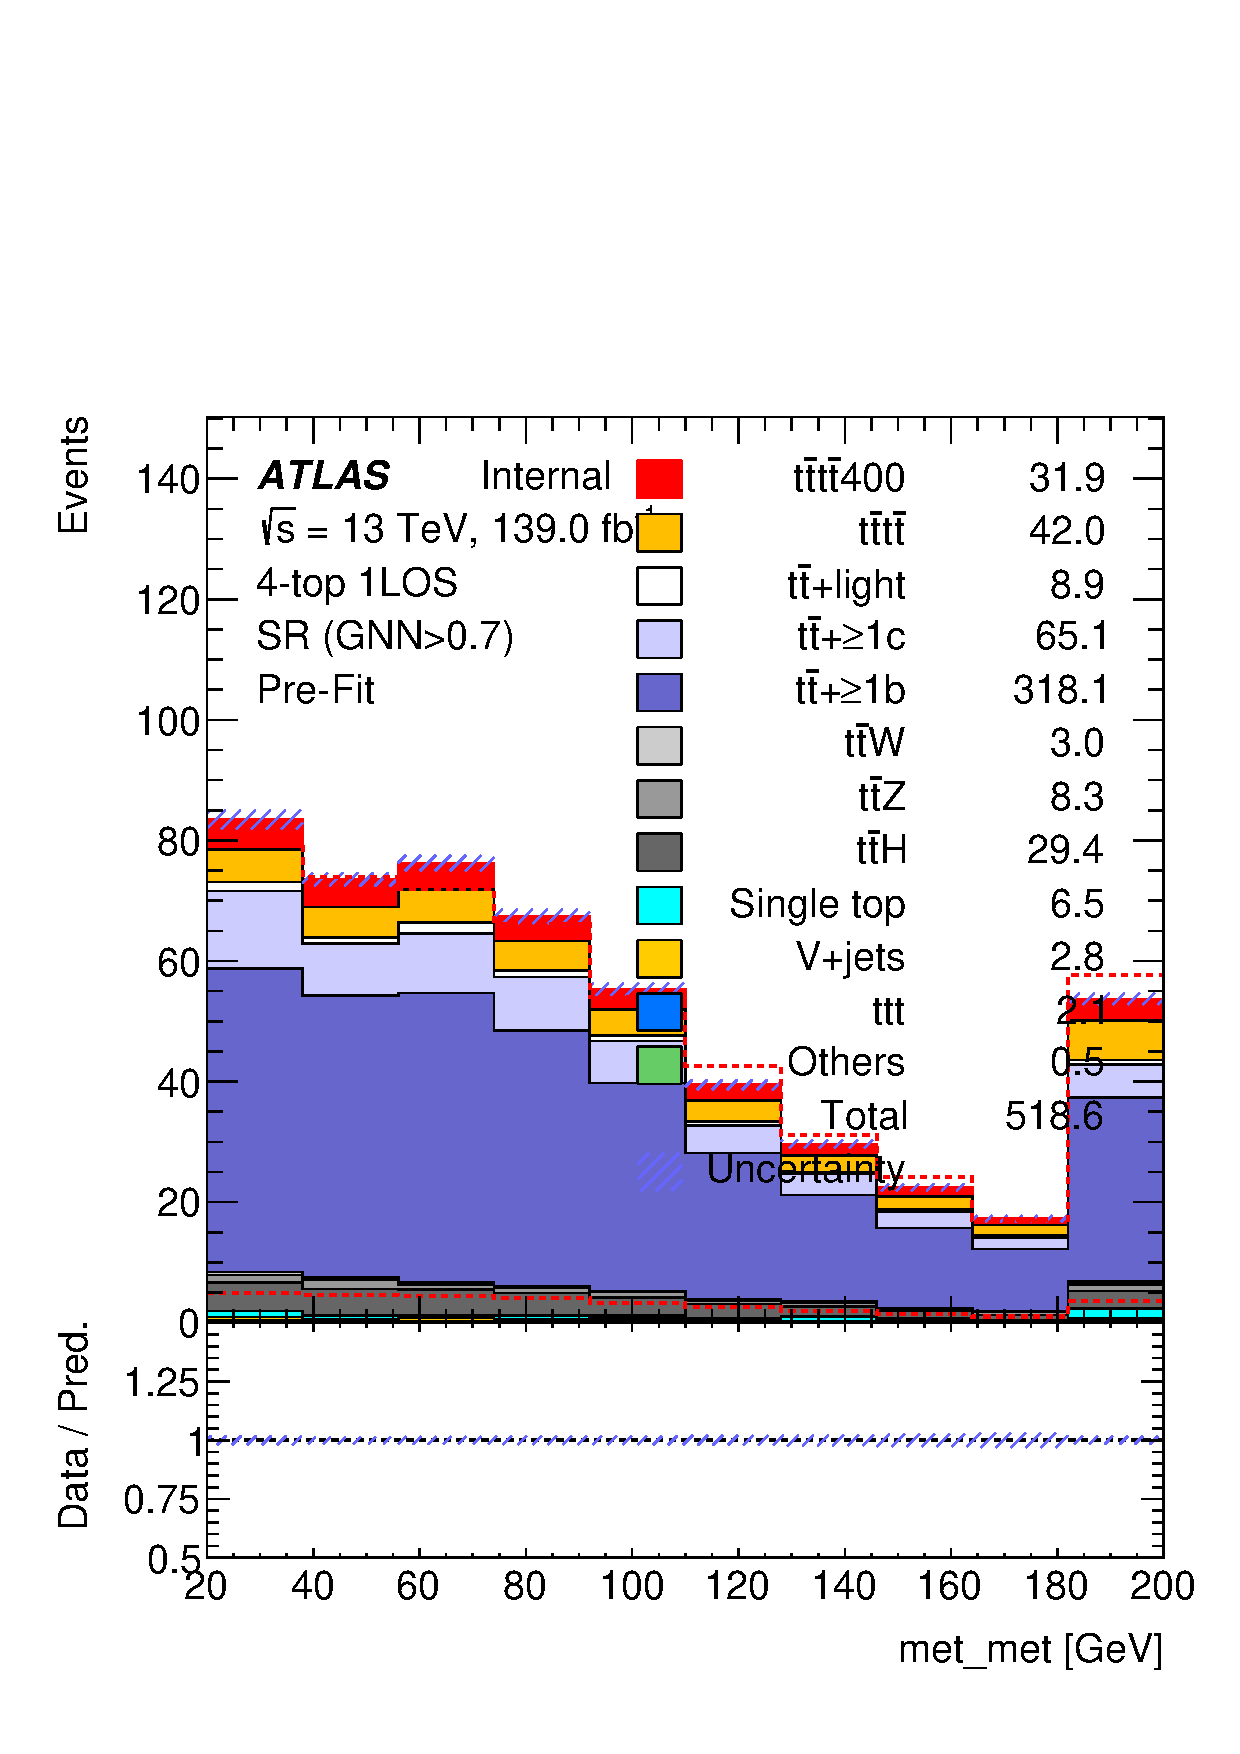
\includegraphics[width=0.23 \textwidth]{figures/gnn/Modeling/met_met.pdf} \\

        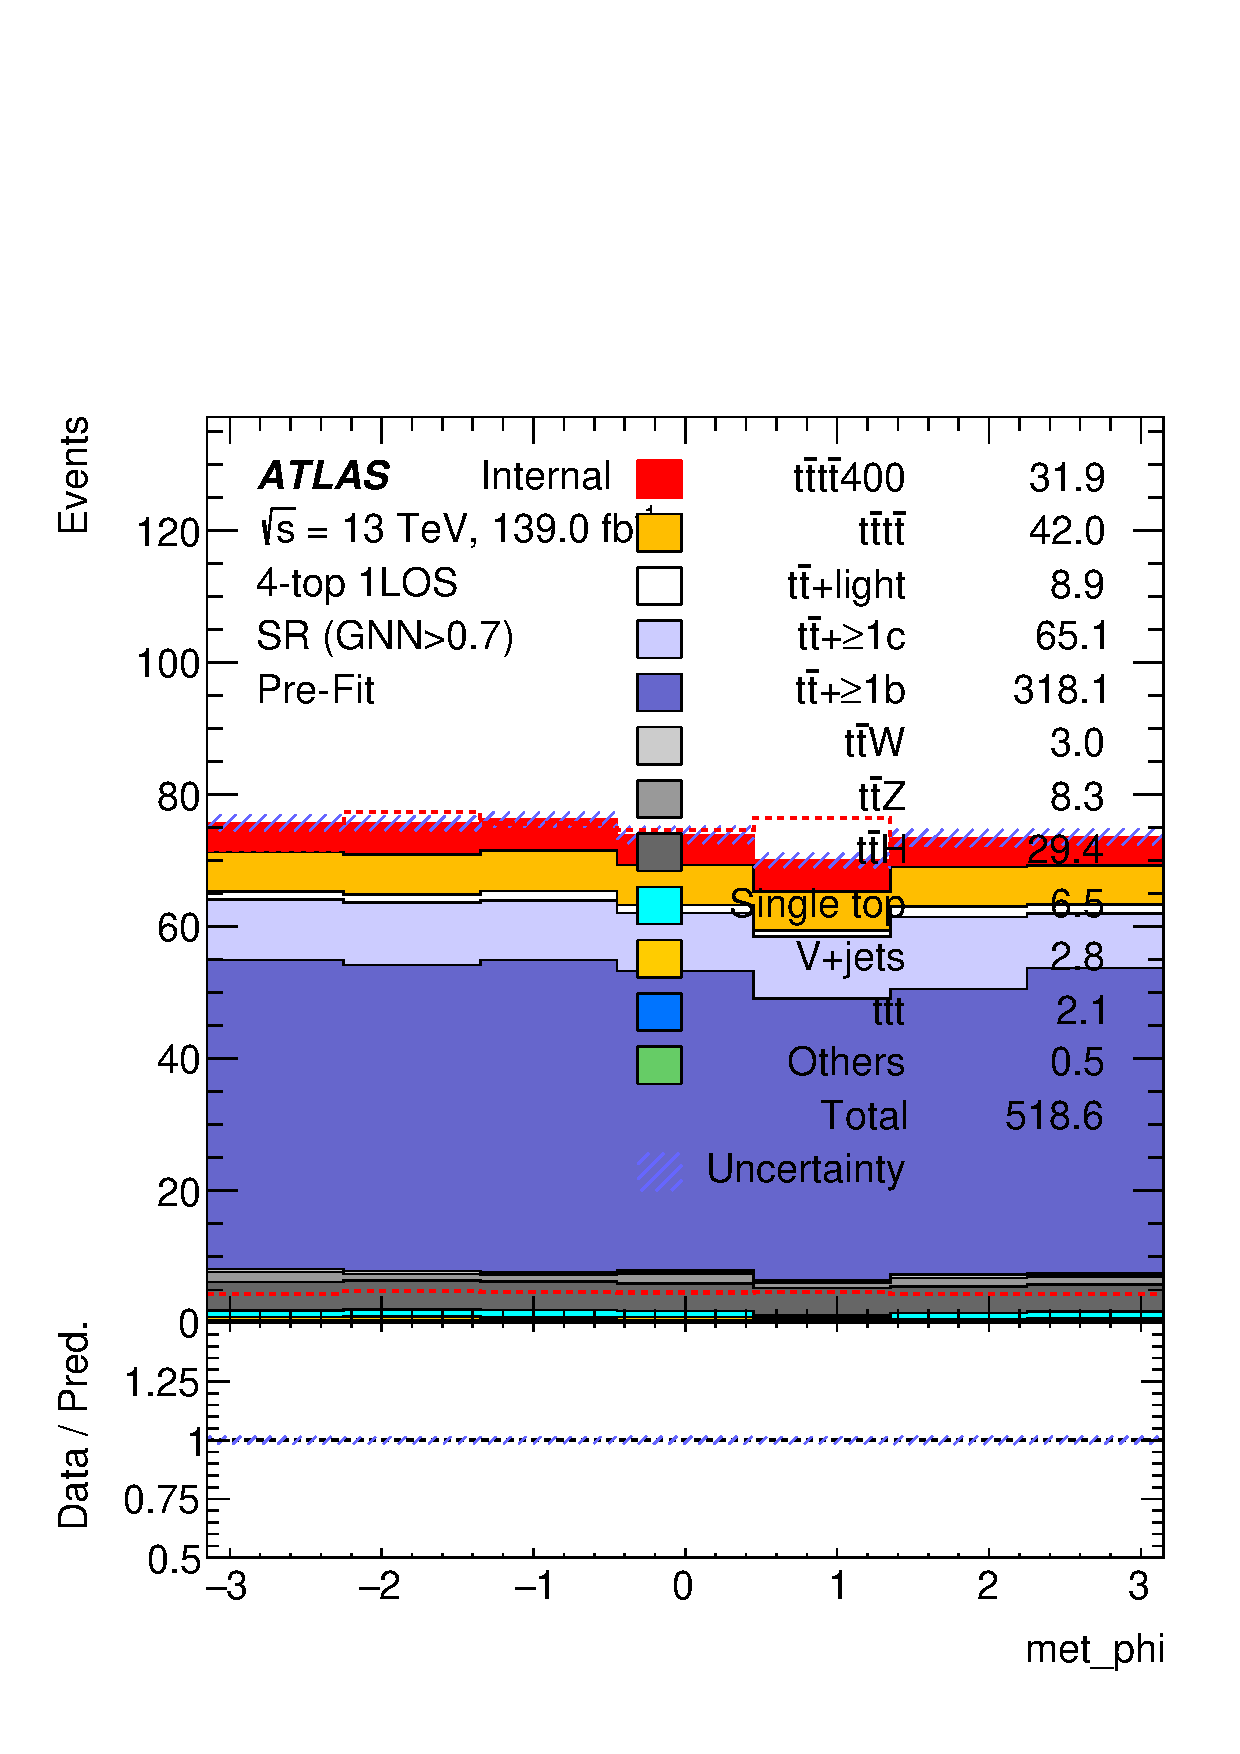
\includegraphics[width=0.23 \textwidth]{figures/gnn/Modeling/met_phi.pdf} &
        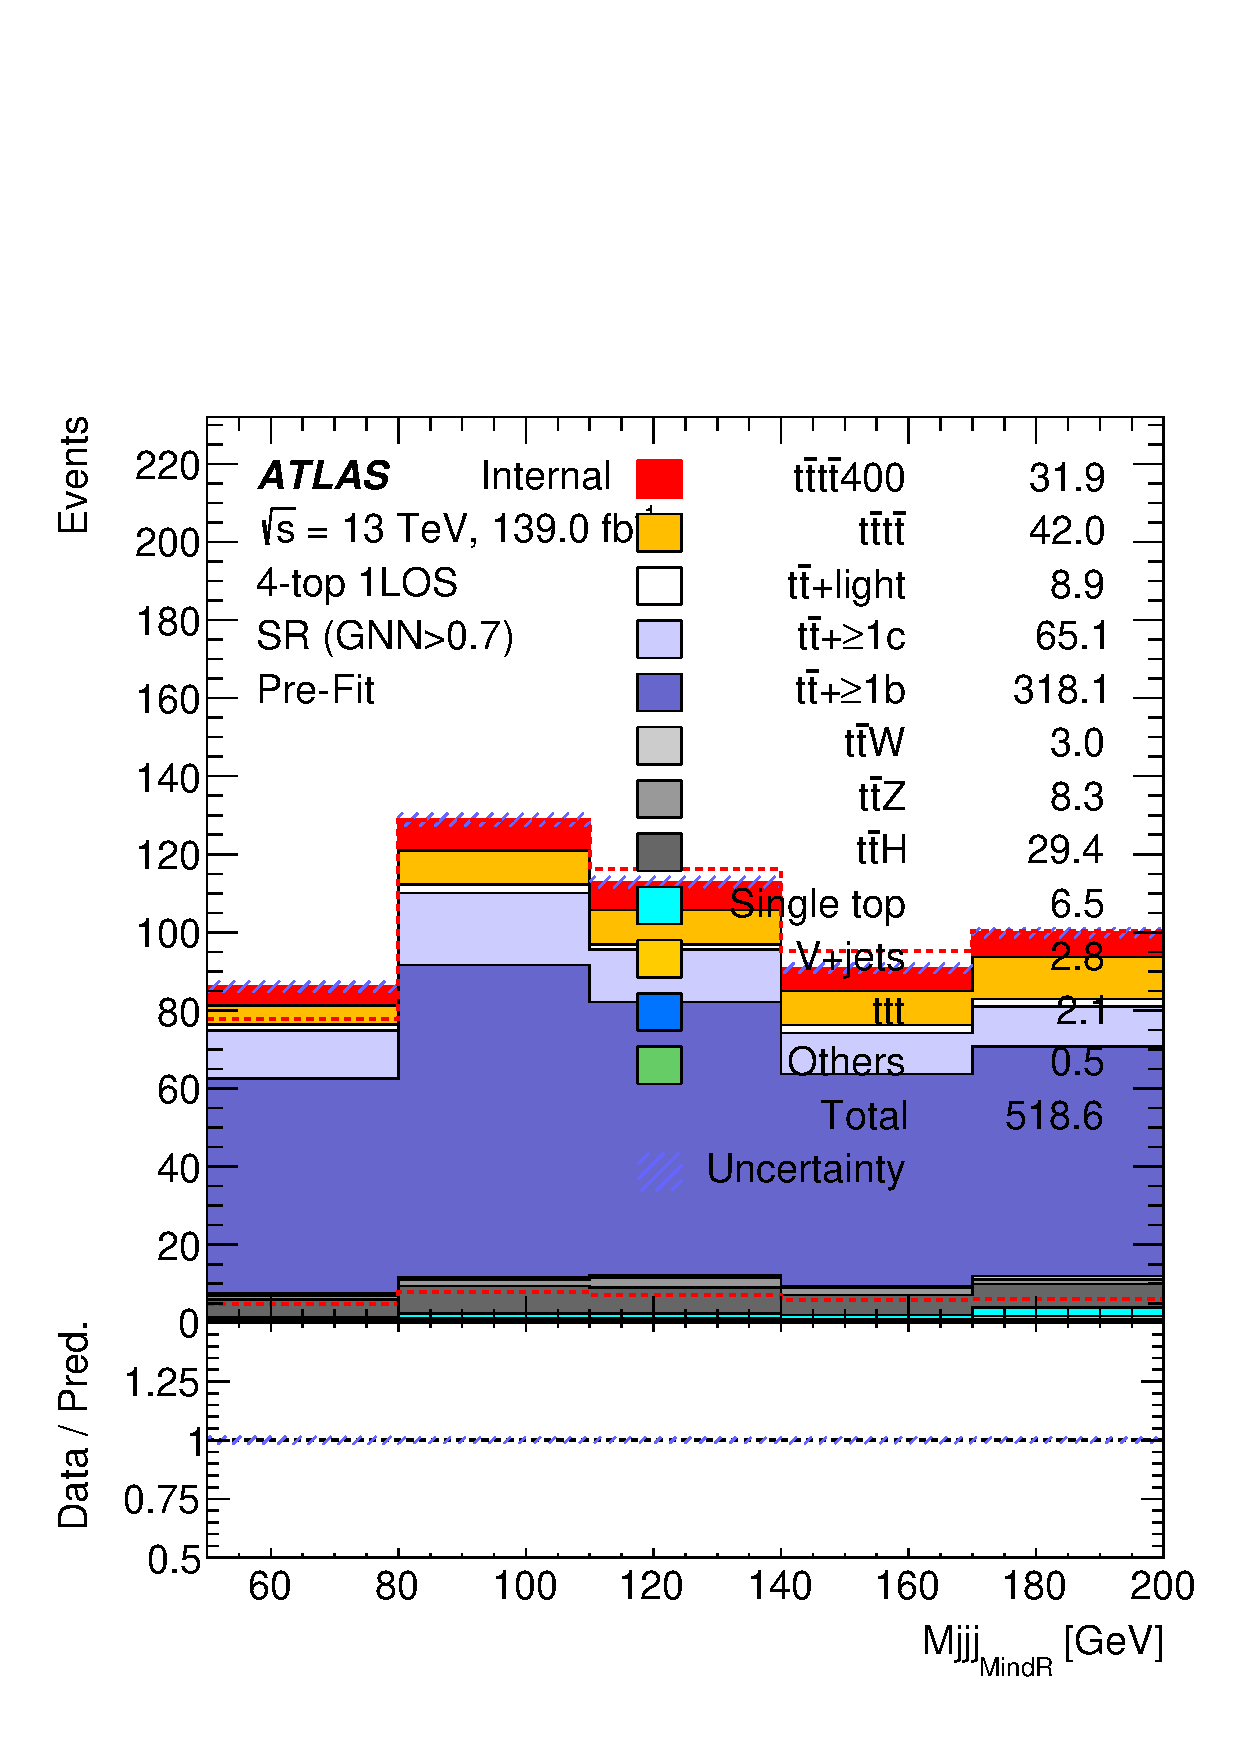
\includegraphics[width=0.23 \textwidth]{figures/gnn/Modeling/Mjjj_MindR.pdf} &
        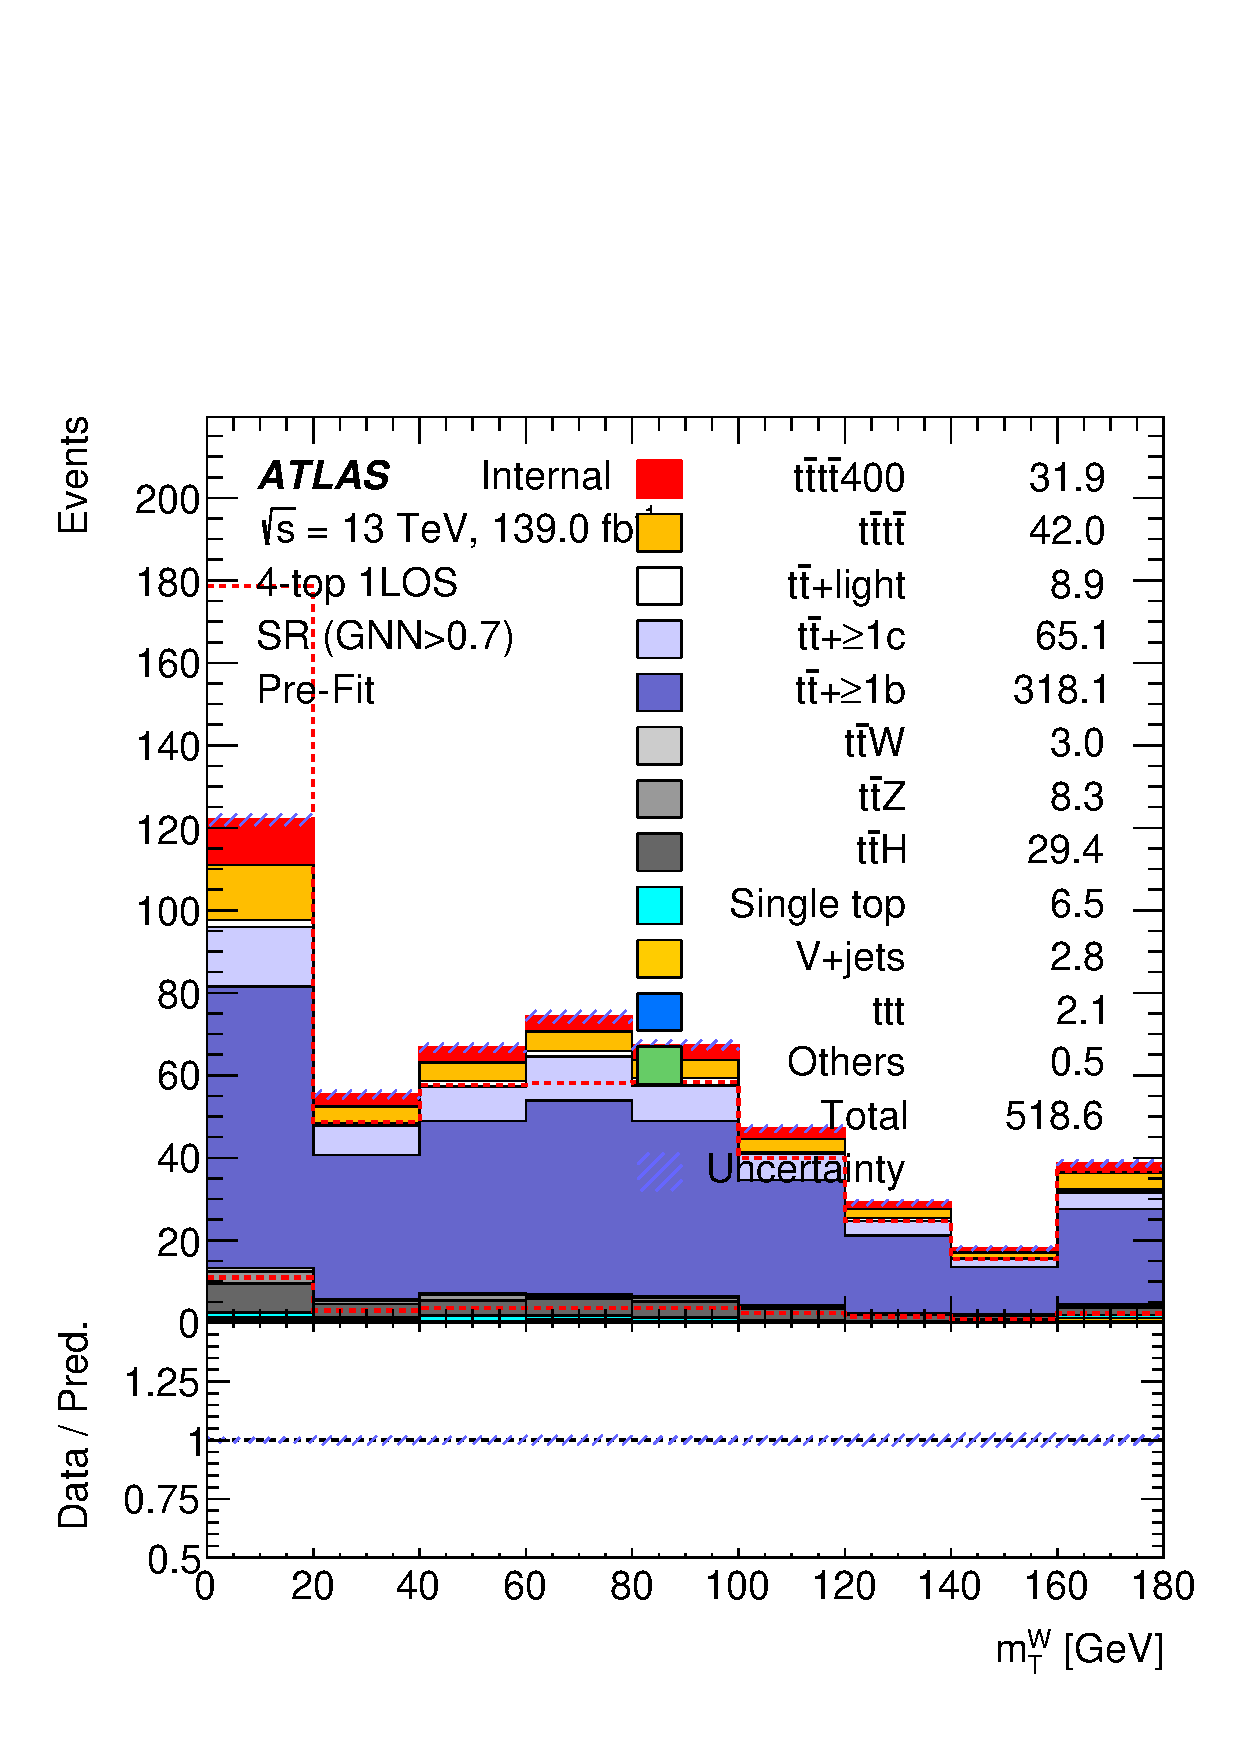
\includegraphics[width=0.23 \textwidth]{figures/gnn/Modeling/mtw.pdf} &
        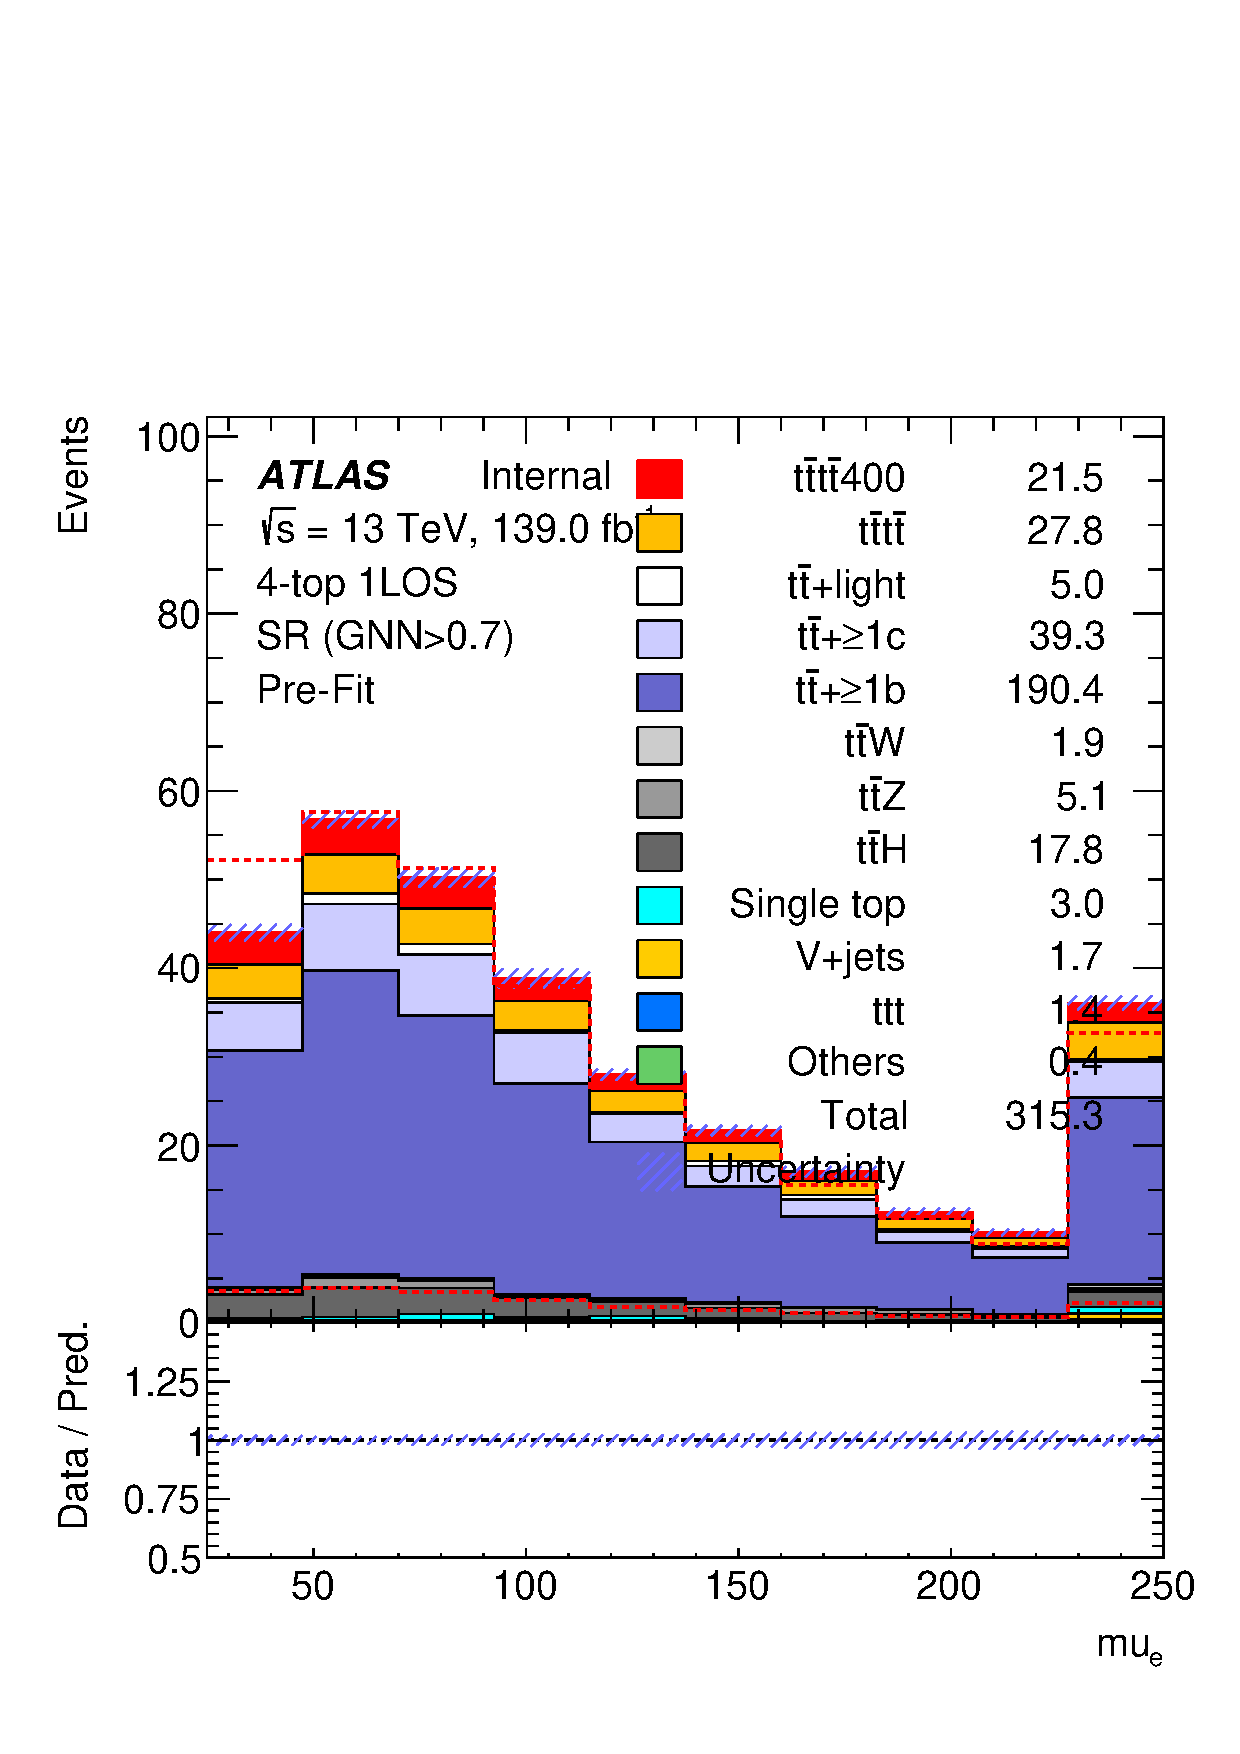
\includegraphics[width=0.23 \textwidth]{figures/gnn/Modeling/mu_e.pdf} \\

        \end{tabular}
        \end{center}

\caption{\label{GNN_input_modelling_1}Distributions for GNN input variables in the inclusive signal region with cut GNN-score>0.7.}
\end{figure}

\begin{figure}

        \begin{center} \setlength{\tabcolsep}{2.5pt}\footnotesize
        \begin{tabular}{cccc}
        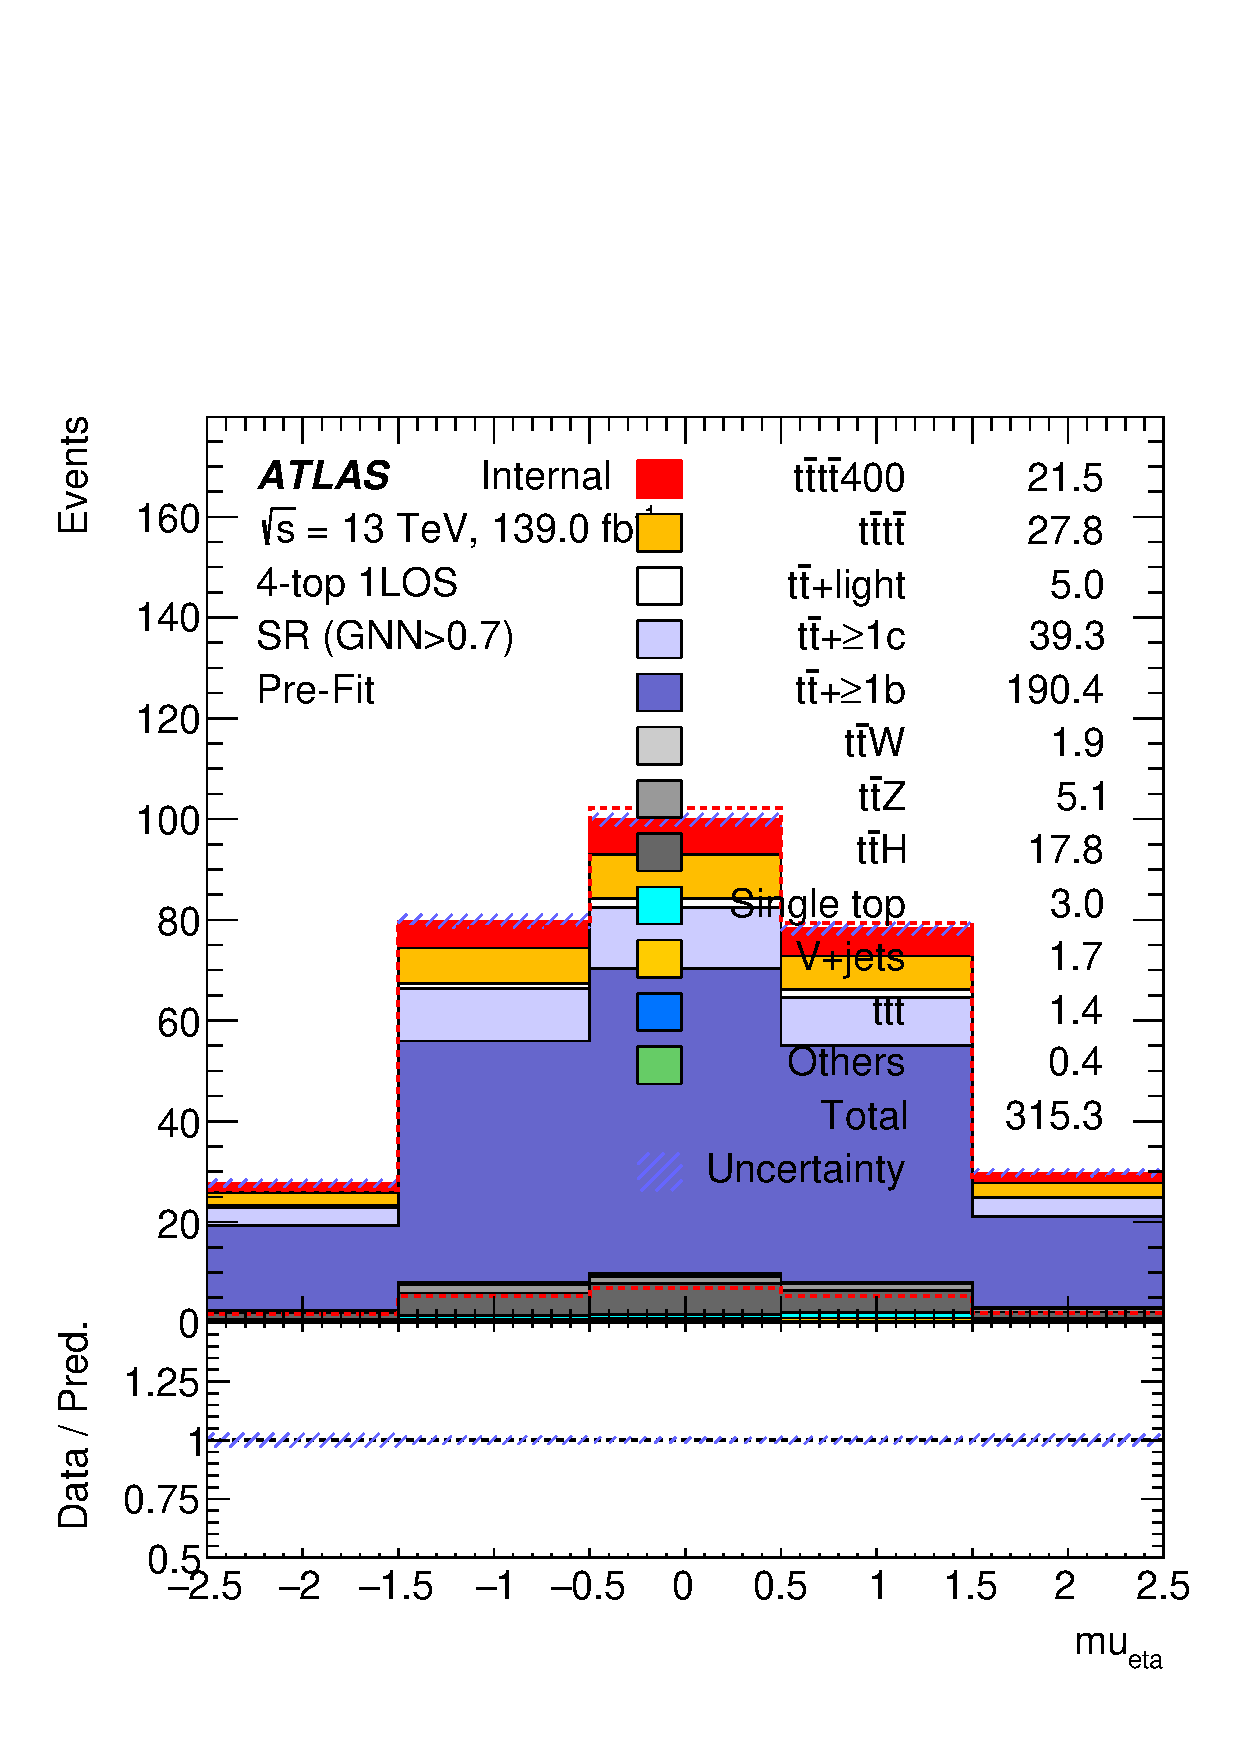
\includegraphics[width=0.23 \textwidth]{figures/gnn/Modeling/mu_eta.pdf} &
        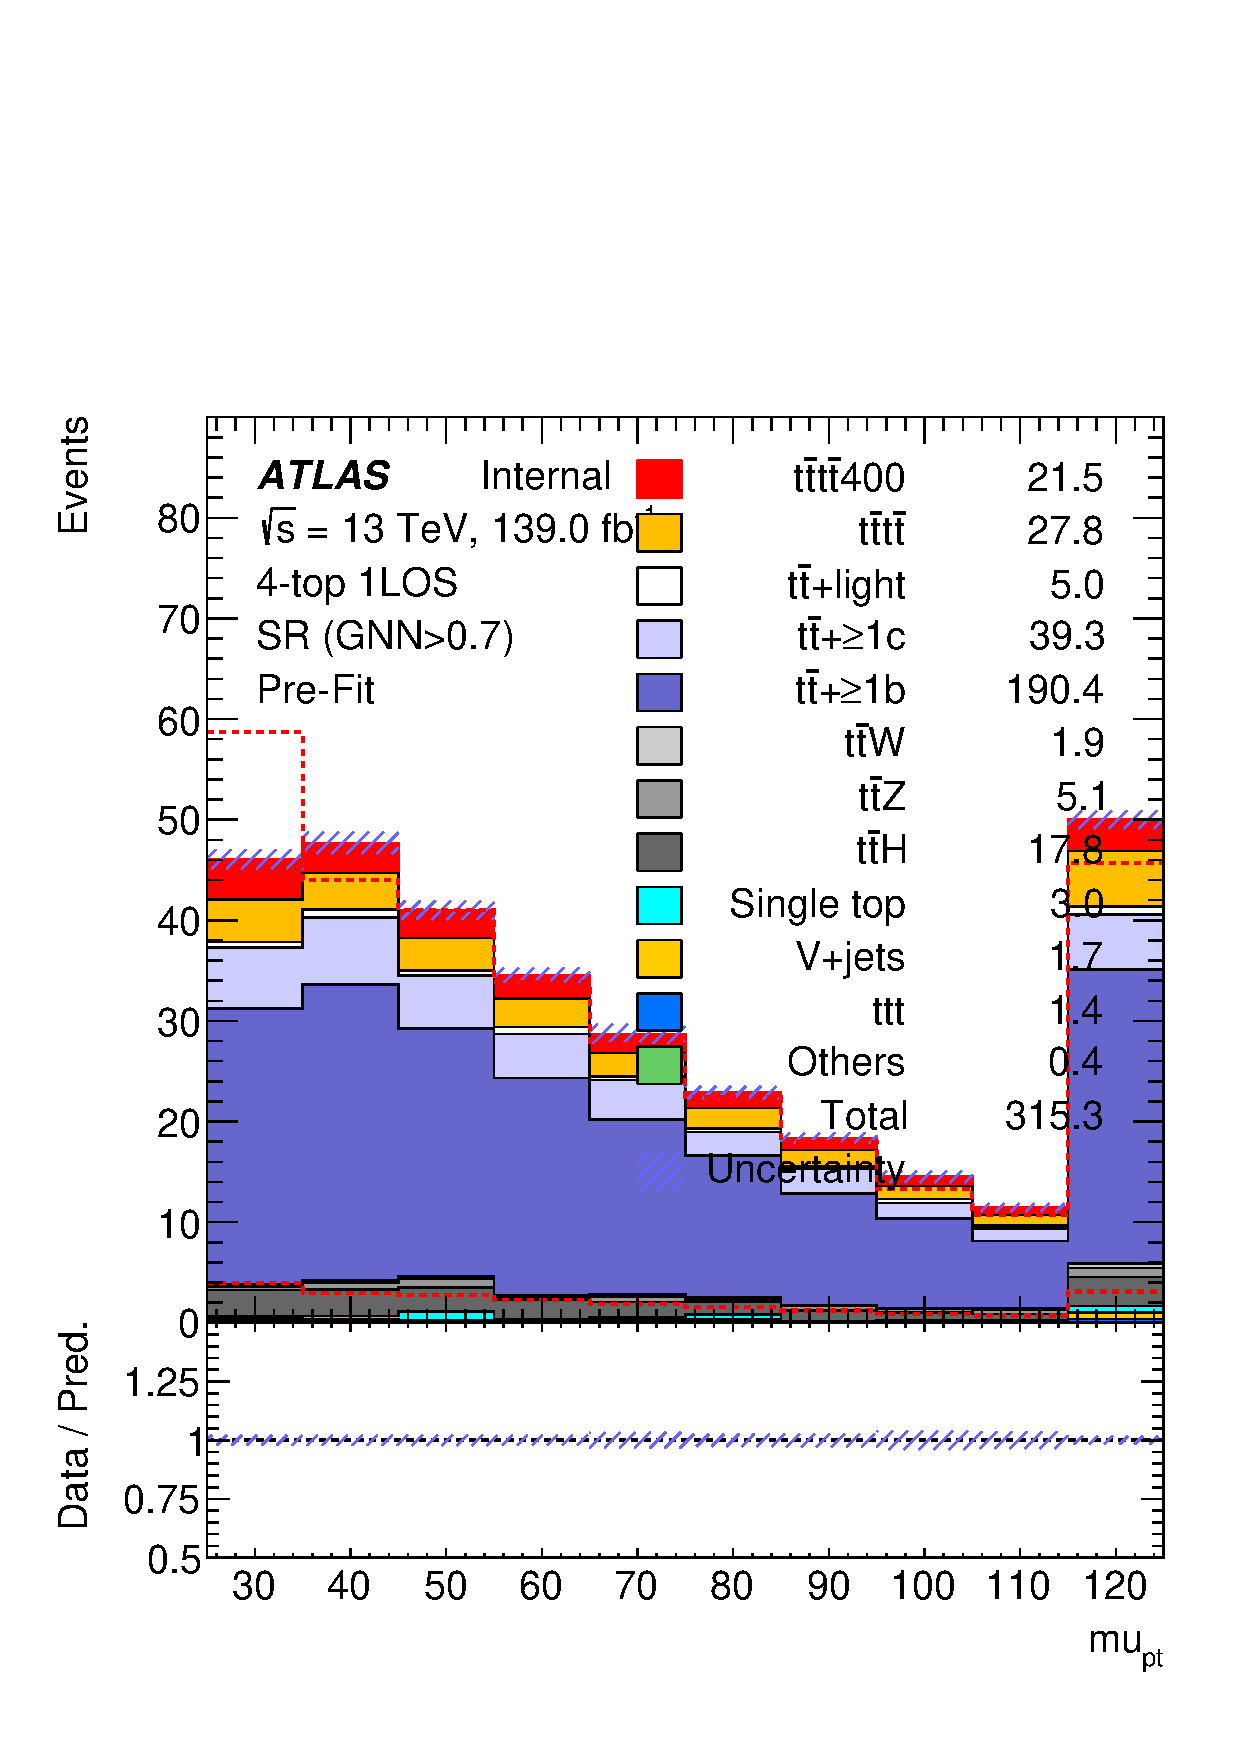
\includegraphics[width=0.23 \textwidth]{figures/gnn/Modeling/mu_pt.pdf} &
        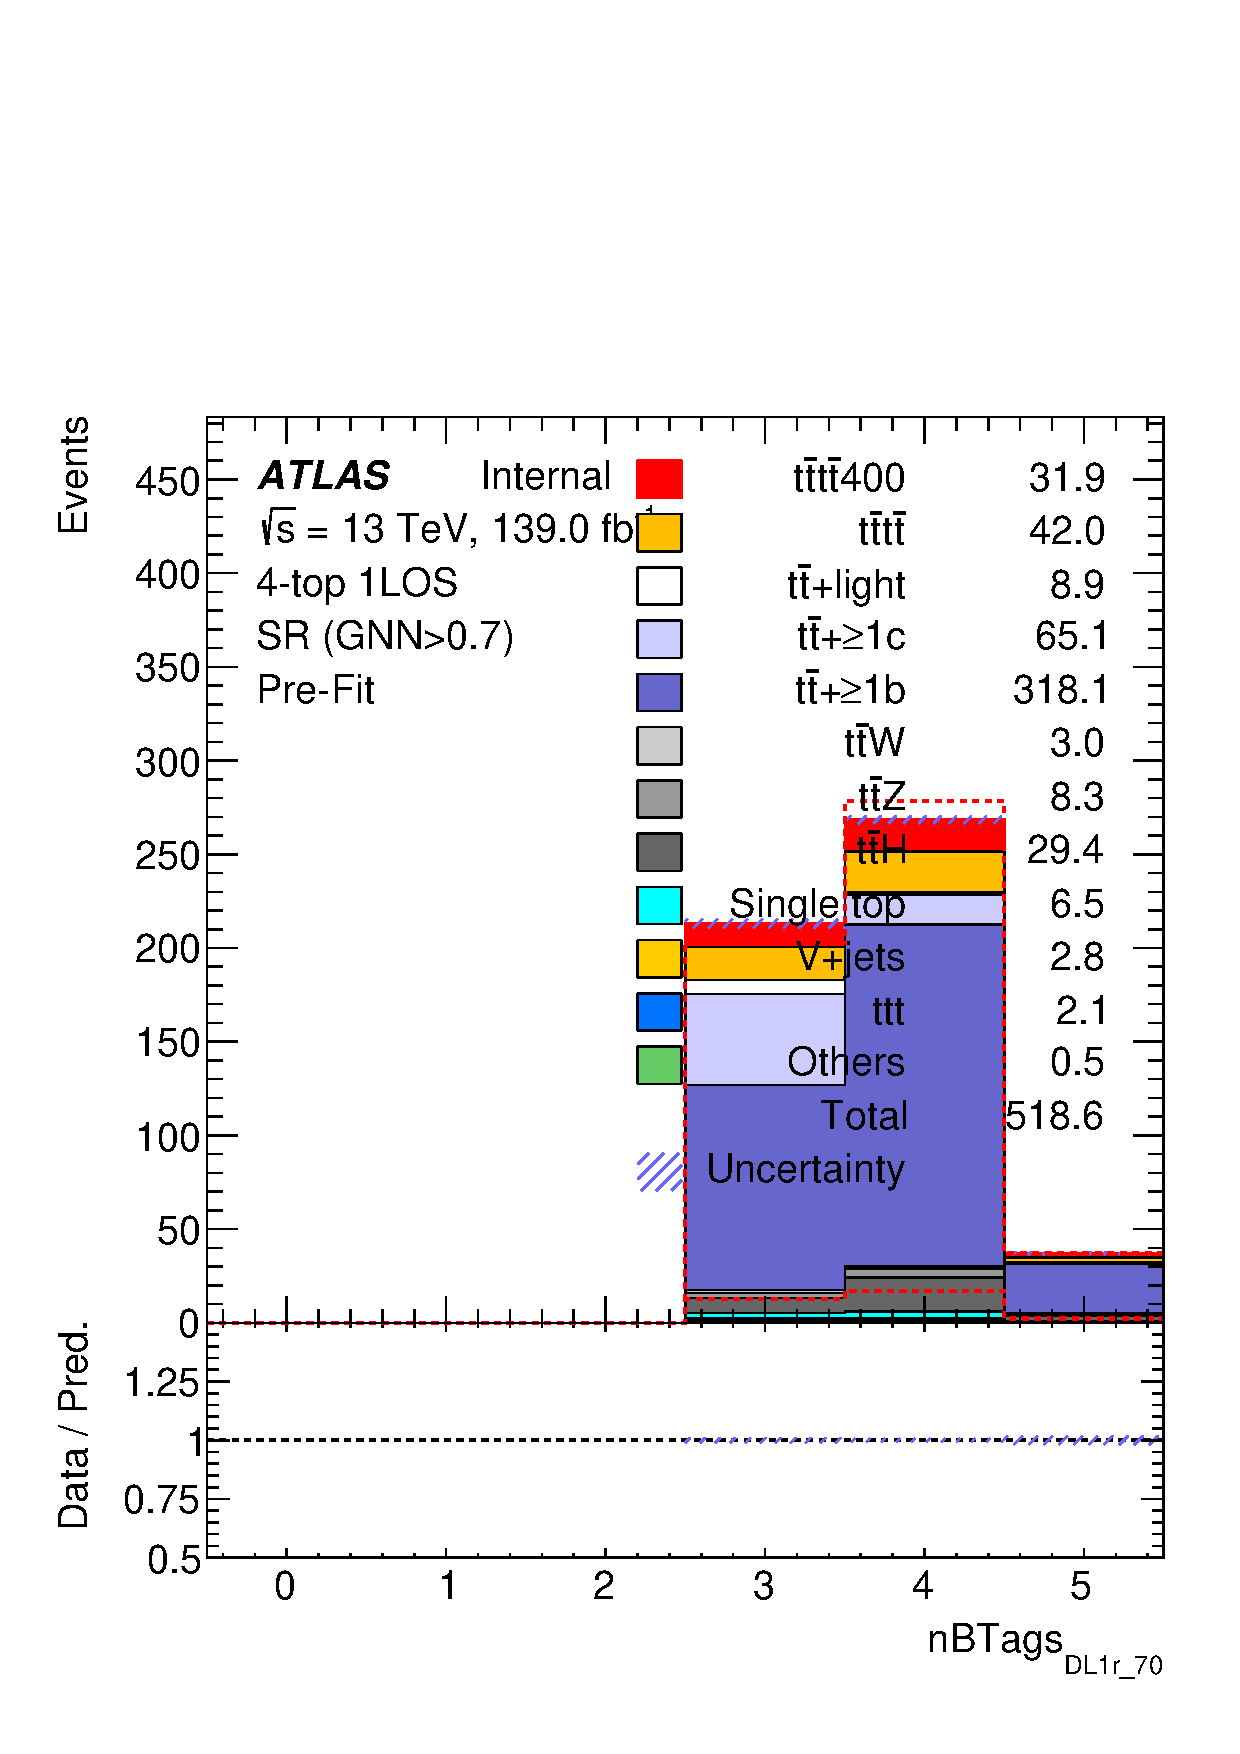
\includegraphics[width=0.23 \textwidth]{figures/gnn/Modeling/nBTags_DL1r_70.pdf} &
        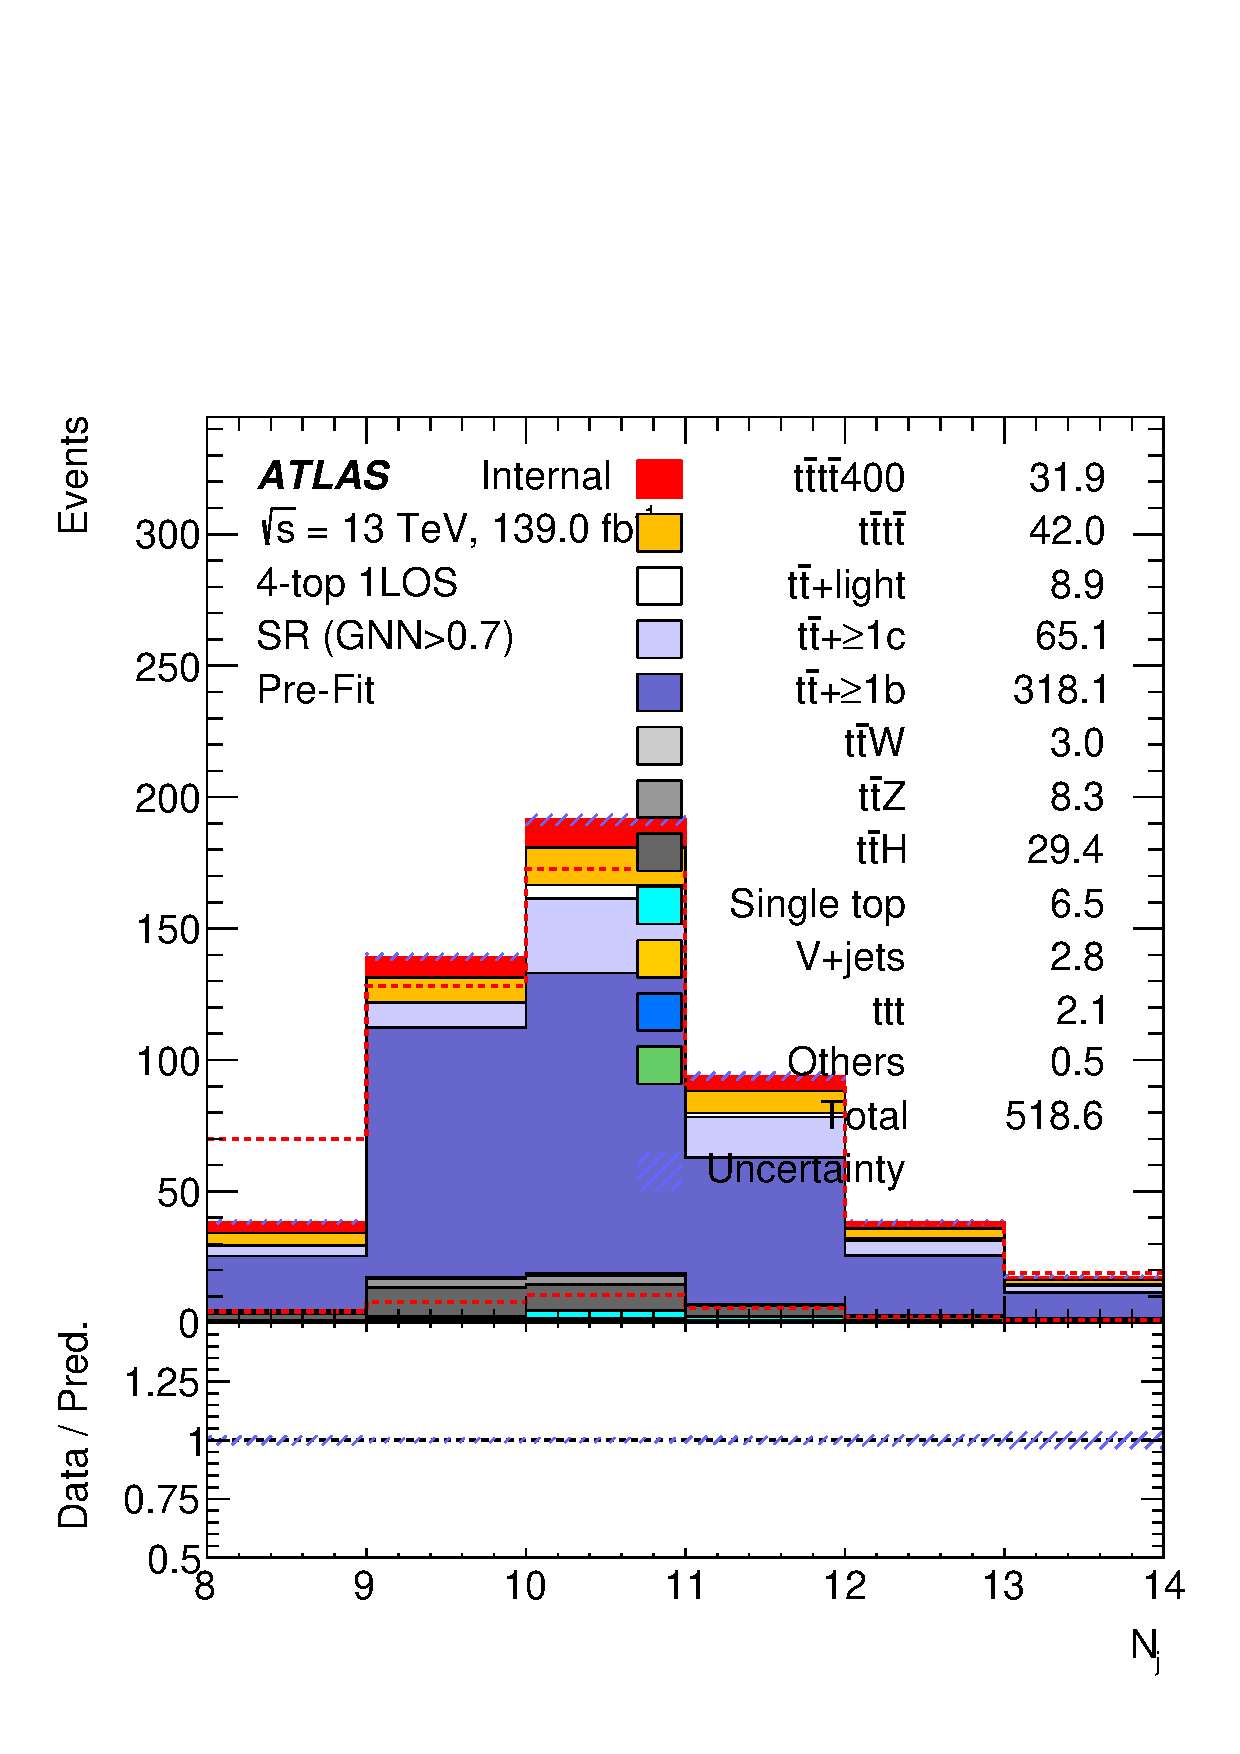
\includegraphics[width=0.23 \textwidth]{figures/gnn/Modeling/nJets.pdf}\\


        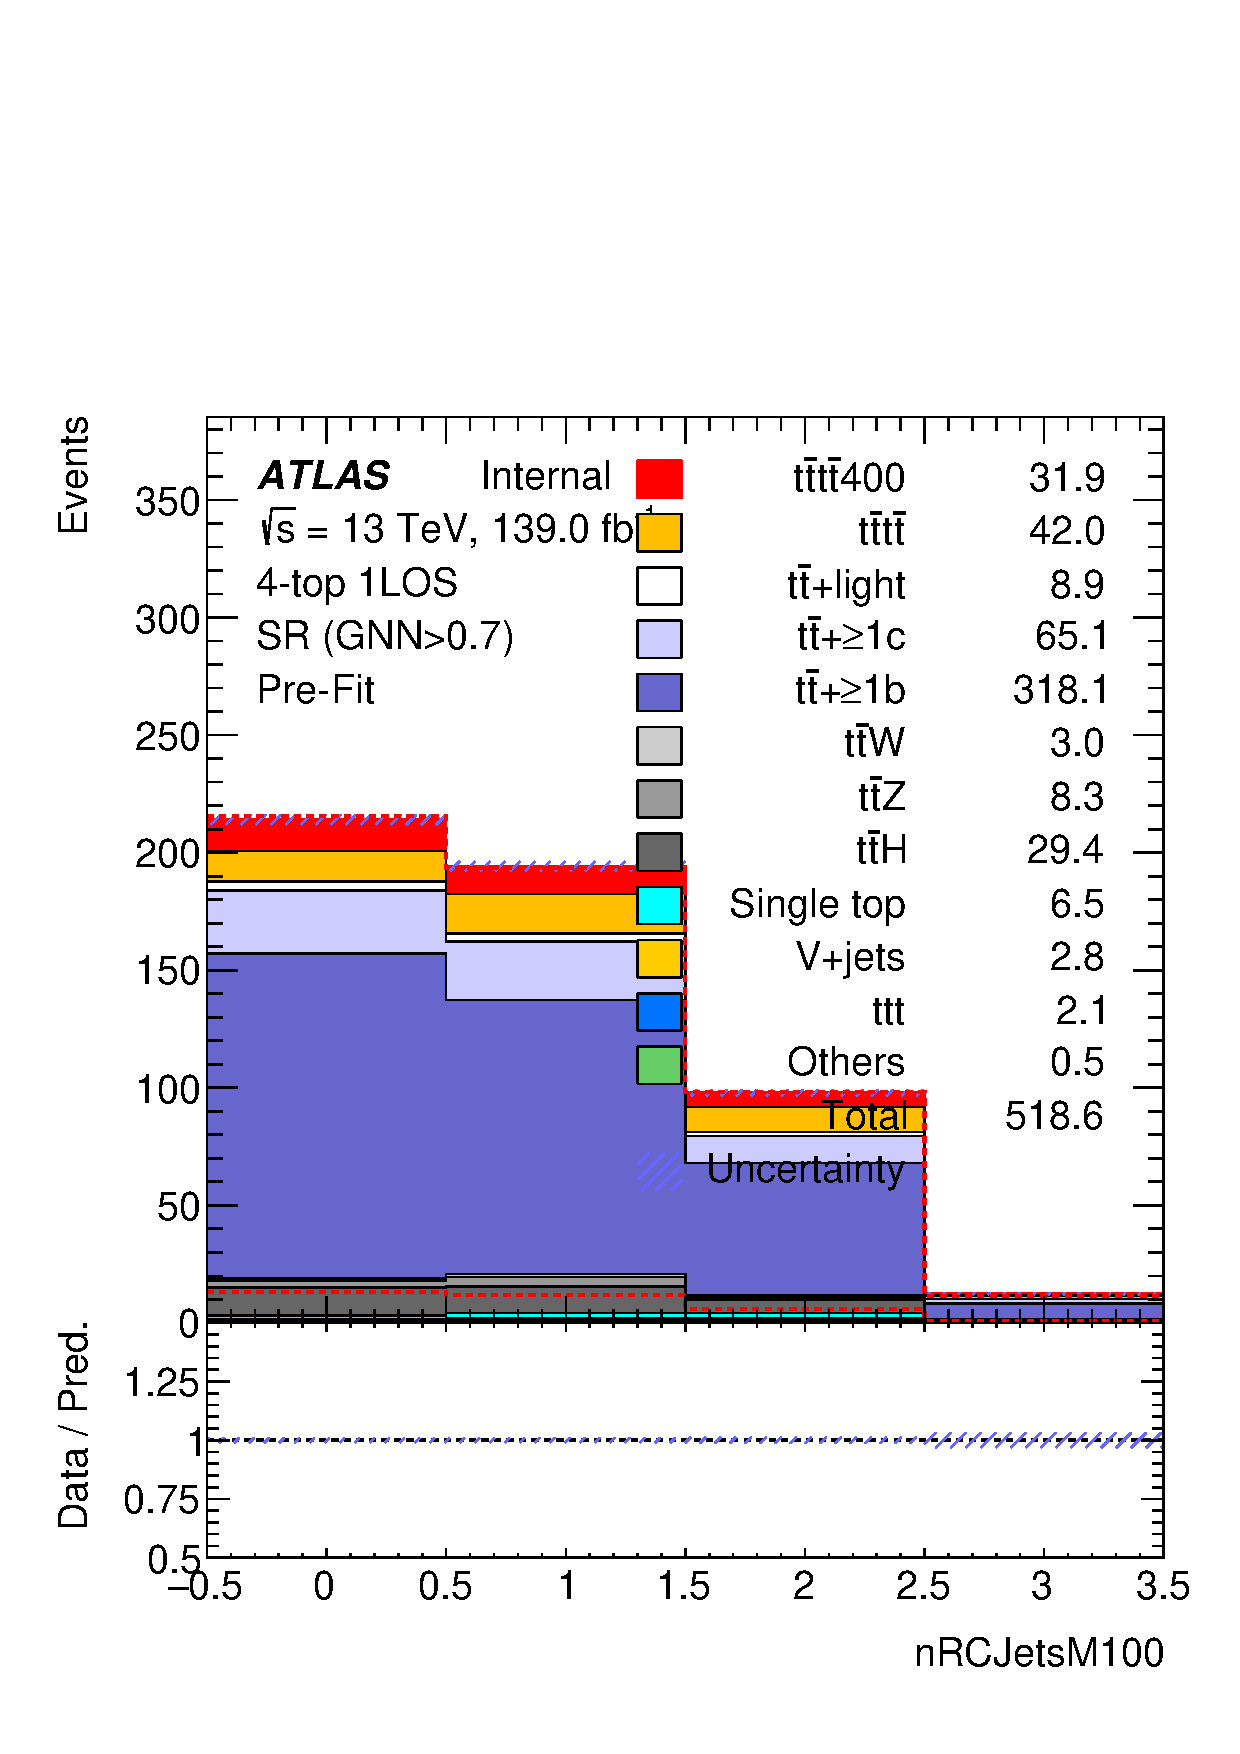
\includegraphics[width=0.23 \textwidth]{figures/gnn/Modeling/nRCJetsM100.pdf} &
        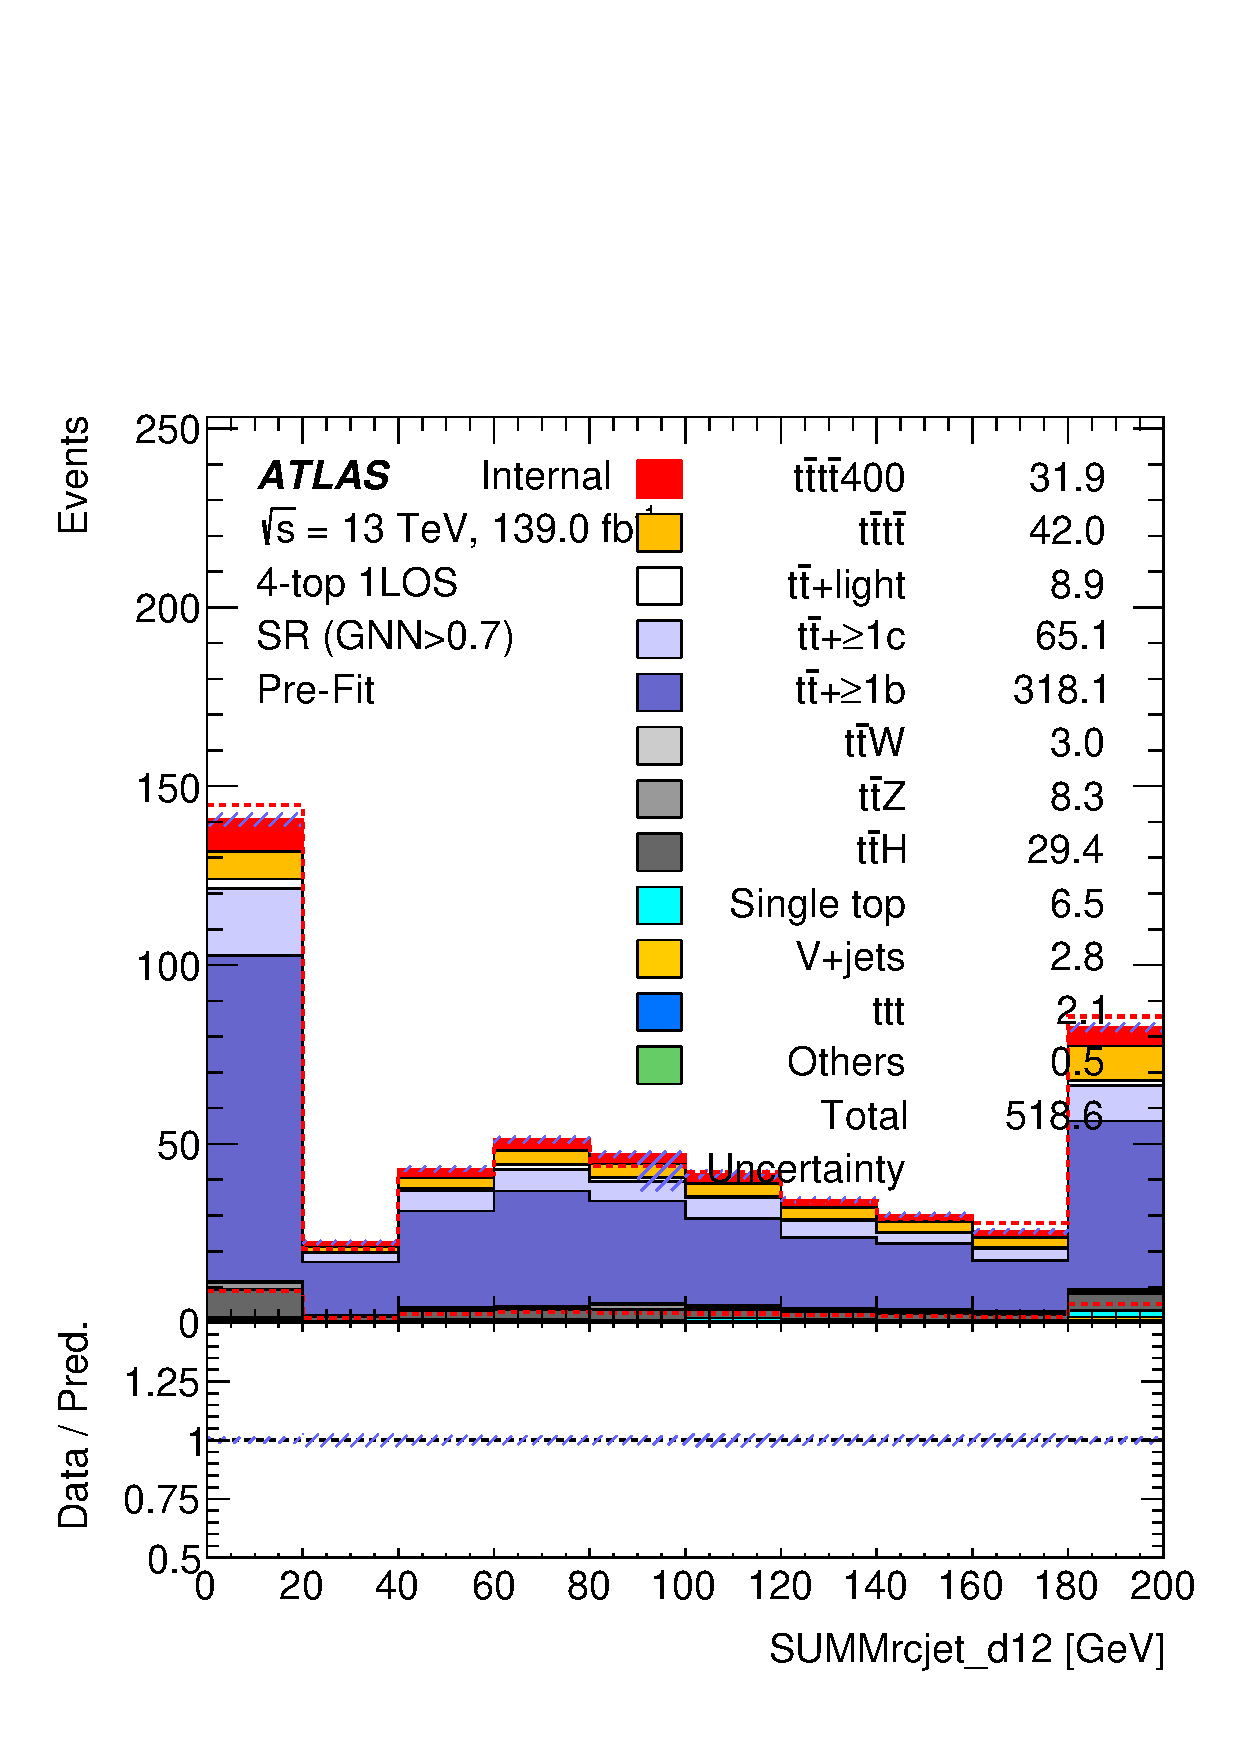
\includegraphics[width=0.23 \textwidth]{figures/gnn/Modeling/sum_d12.pdf} &
        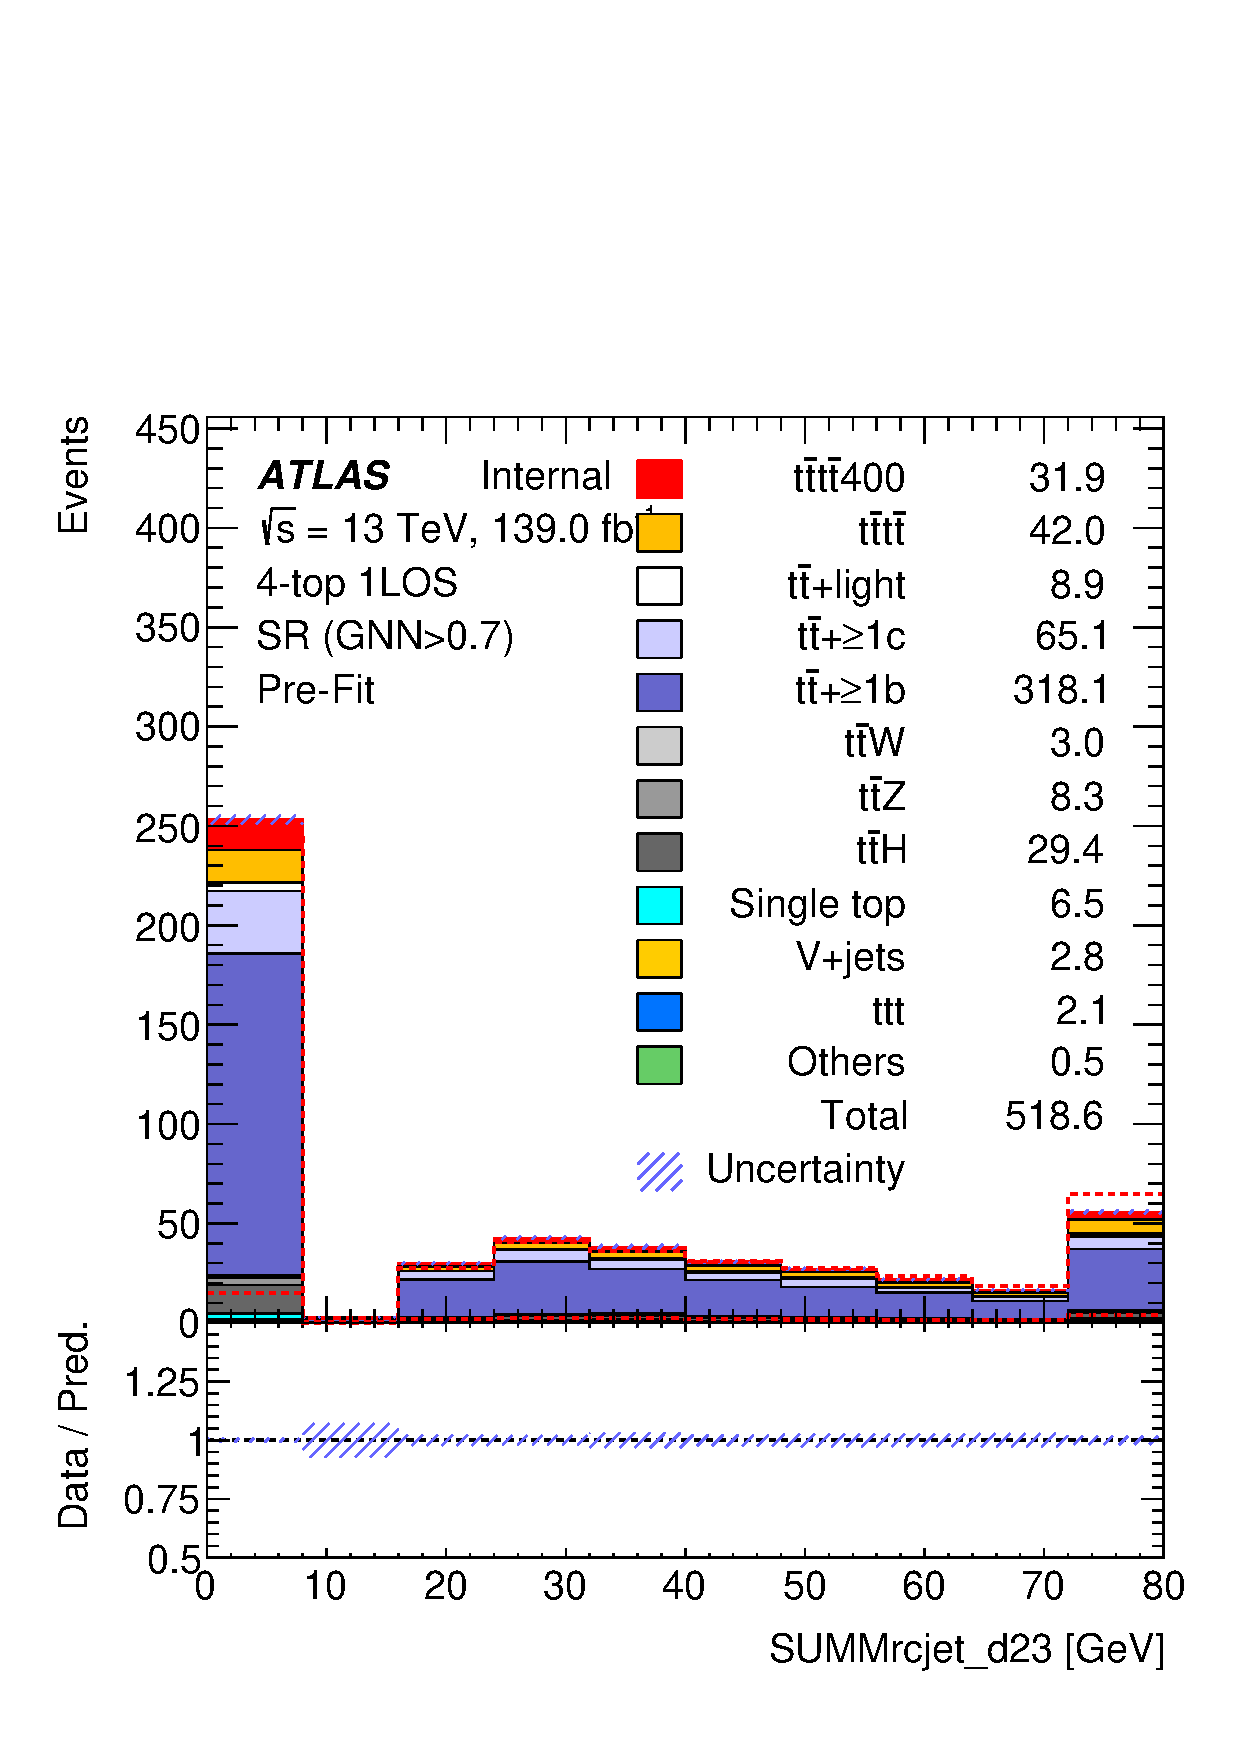
\includegraphics[width=0.23 \textwidth]{figures/gnn/Modeling/sum_d23.pdf} &
        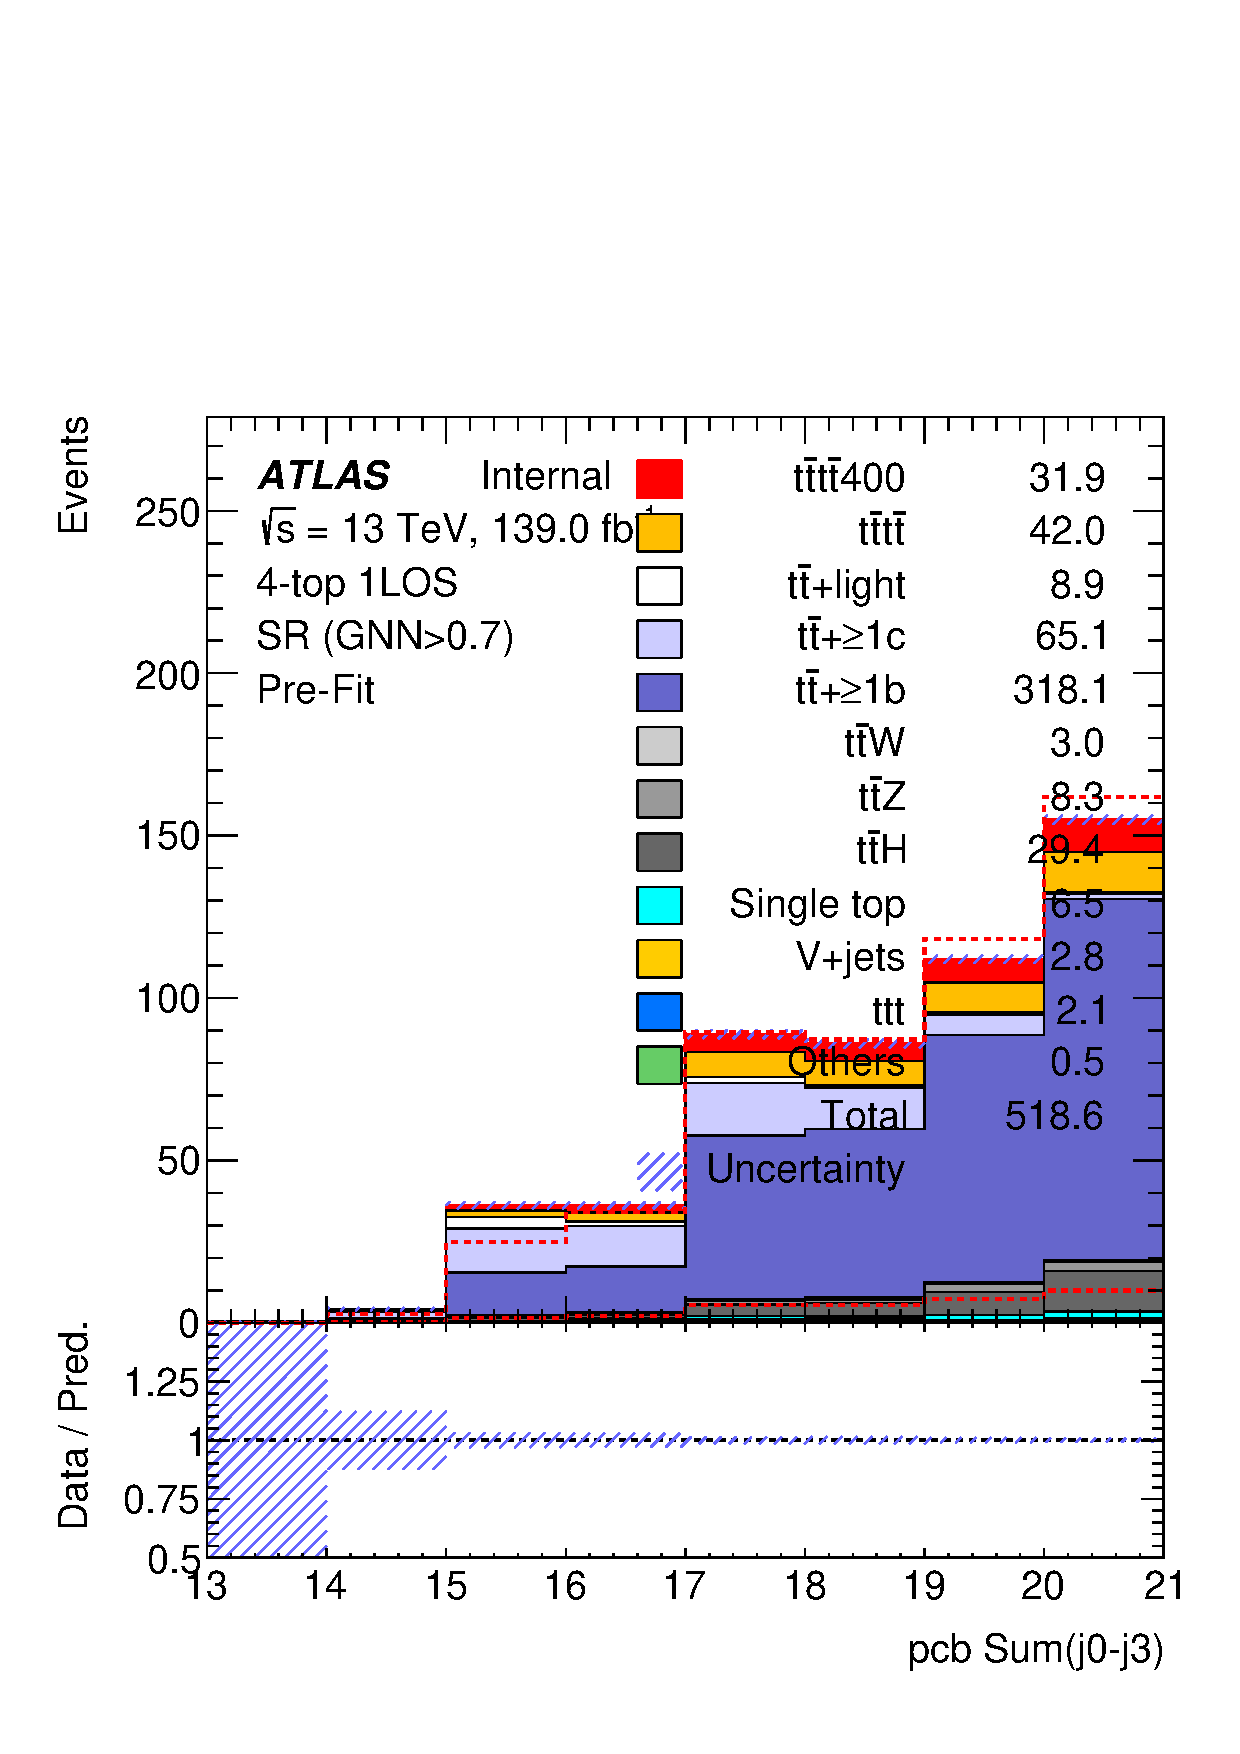
\includegraphics[width=0.23 \textwidth]{figures/gnn/Modeling/pcb.pdf} \\


        \end{tabular}
        \end{center}

\caption{\label{GNN_input_modelling_2}Distributions for GNN input variables in the inclusive signal region with cut GNN-score>0.7.}
\end{figure}
